% TODO (master-document merge): this file is compiled standalone as `article`,
% with \section standing in for what will become \chapter once the thesis is
% assembled. Chapter 1 (chapter1_introduction.tex) is in the same standalone
% state for the same reason. Converting a single chapter to `report`/\chapter
% now, while its sibling remains `article`/\section, would leave the two
% chapters structurally inconsistent with each other until both are merged.
% At merge time: switch \documentclass to `report` (or `book`), replace this
% file's top-level \section with \chapter and demote \subsection -> \section,
% \subsubsection -> \subsection accordingly, apply the same demotion to every
% other chapter file, and move all six \begin{thebibliography} blocks into a
% single shared bibliography (a .bib file via BibTeX/biblatex, or one merged
% thebibliography) so each chapter stops carrying its own duplicate reference
% list. All \ref/\label numbering (Section 2.1, 2.2, ... and the "Section 1.X"
% cross-references into Chapter 1 already written throughout this file) will
% resolve automatically to the correct chapter-relative numbers once this is
% done; no cross-reference text needs to change by hand.
\documentclass[11pt, a4paper, twoside]{article}

\usepackage[utf8]{inputenc}
\usepackage[a4paper, left=1.5in, right=1.5in, top=1in, bottom=1in]{geometry}
\usepackage{amsmath, amssymb, amsfonts}
\usepackage{textcomp}
\usepackage{booktabs, tabularx, array}
\usepackage{graphicx, caption, subcaption}
\usepackage[hidelinks]{hyperref}
\usepackage{natbib}
\bibliographystyle{plainnat}
\usepackage{newtxtext, newtxmath}
\usepackage{setspace}
\onehalfspacing

\title{\textbf{Chapter 2 --- Methodology and Empirical Wind-Speed Modelling}\\[4pt]
\large Continuous-Time Modelling of Wind Speed for Derivatives Pricing and Risk Management}
\author{}
\date{}

\begin{document}

\maketitle

This chapter develops the wind-speed modelling pipeline whose motivation and literature grounding were set out in Chapter~1: a five-stage sequence running from deseasonalisation through discrete-time autoregression and conditional volatility to a continuous-time embedding and, finally, a theoretical stochastic-volatility extension. Each stage is applied identically to both datasets described in Section~1.4: Dataset A (Bologna, 10~m, 2015--2018), on which the pipeline is developed and validated, and Dataset B (Nordfriesland, 100~m, 2015--2024), which carries the thesis's headline results. Each section below presents the two datasets side by side, so that methodological choices can be compared directly against the data they are applied to. Numerical results quoted throughout are frozen outputs of the underlying phase notebooks; none are re-estimated here.

\section{Deseasonalisation and the Box--Cox Transformation}
\label{sec:phase1}

Raw daily wind speed is a positive, right-skewed, seasonally heteroskedastic quantity, and every subsequent stage of this pipeline (the AR(4) mean model of Section~\ref{sec:phase2}, the GARCH(1,1) volatility layer of Section~\ref{sec:phase3}, and the CAR(4) continuous-time embedding of Section~\ref{sec:phase4}) presupposes a series that is approximately Gaussian, zero-mean, and unit-variance. The first stage of the pipeline is therefore a sequence of four operations applied to raw wind speed $W(t)$: characterising its marginal distribution, applying a Box--Cox power transformation, removing a deterministic seasonal mean $\Lambda(t)$ via a truncated Fourier series, and removing a deterministic seasonal variance $\sigma^2(t)$ via a second Fourier fit. The output is the standardised series $\widetilde W(t) = [W^{(\lambda)}(t) - \Lambda(t)]/\sigma(t)$, which enters the AR(4) model of Section~\ref{sec:phase2}.

\subsection{Marginal Distribution}
\label{sec:phase1-marginal}

The two marginal distributions fitted throughout this section are the Weibull and the lognormal,
\begin{align}
f_W(v;k,c) &= \frac{k}{c}\left(\frac{v}{c}\right)^{k-1}\exp\left[-\left(\frac{v}{c}\right)^k\right],\ v \geq 0, \\
f_L(v;m,s) &= \frac{1}{vs\sqrt{2\pi}}\exp\left[-\frac{(\ln v - m)^2}{2s^2}\right],\ v > 0,
\end{align}
both fitted by maximum likelihood and compared by Akaike information criterion. Table~\ref{tab:weibull-fit} reports the resulting fits for both datasets. \citet{TullerBrett1984} provide the physical justification for the Weibull distribution reviewed in Section~1.3.1: under approximate bivariate-normal isotropy of the horizontal wind-velocity components, wind speed is Weibull-distributed with shape parameter near two. Dataset B, measured at 100~m in the free atmosphere above the surface boundary layer, conforms to this picture: the Weibull distribution ($\hat k = 2.67$) beats the lognormal alternative on both AIC and BIC, consistent with \citet{TullerBrett1984} and with the case-study evidence of \citet{Garcia1998}. Dataset A does not: at 10~m, where surface friction and diurnal boundary-layer cycling distort the isotropy assumption underlying the Weibull derivation, the lognormal distribution wins decisively (log-likelihood $-1{,}730.6$ versus $-1{,}960.5$ for the Weibull MLE fit, $\Delta\text{AIC} \approx 460$). This is the same qualitative finding already noted in Section~1.4.1; it is repeated here because it is the reason the two datasets receive different treatment in the Box--Cox step that follows.

\begin{table}[htbp]
\centering
\small
\caption{Marginal distribution fits, both datasets (maximum likelihood).}
\label{tab:weibull-fit}
\begin{tabularx}{\textwidth}{l >{\raggedright\arraybackslash}X >{\raggedright\arraybackslash}X}
\toprule
& \textbf{Dataset A} & \textbf{Dataset B} \\
\midrule
Weibull $(\hat k, \hat c)$ & $2.6368$, $2.7729$~m/s & $2.67$, $9.09$~m/s \\
Lognormal $(\hat m, \hat s)$ & $0.8423$, $0.3405$ & $2.00$, $0.43$ \\
Log-likelihood, Weibull & $-1{,}960.51$ & n/a$^{\ast}$ \\
Log-likelihood, Lognormal & $-1{,}730.56$ & n/a$^{\ast}$ \\
AIC, Weibull / Lognormal & $3{,}925.01$ / $3{,}465.12$ & $18{,}758.3$ / $18{,}803.1$ \\
Better fit & \textbf{Lognormal} ($\Delta\text{AIC}\!\approx\!460$) & \textbf{Weibull} ($\Delta\text{AIC}\!\approx\!45$) \\
\bottomrule
\end{tabularx}
\vspace{2pt}
{\footnotesize $^{\ast}$Dataset A's log-likelihoods are reported in the source analysis; Dataset B's own report gives AIC/BIC directly without a separately tabulated log-likelihood column.}
\end{table}

\begin{figure}[htbp]
\centering
\begin{subfigure}{0.48\textwidth}
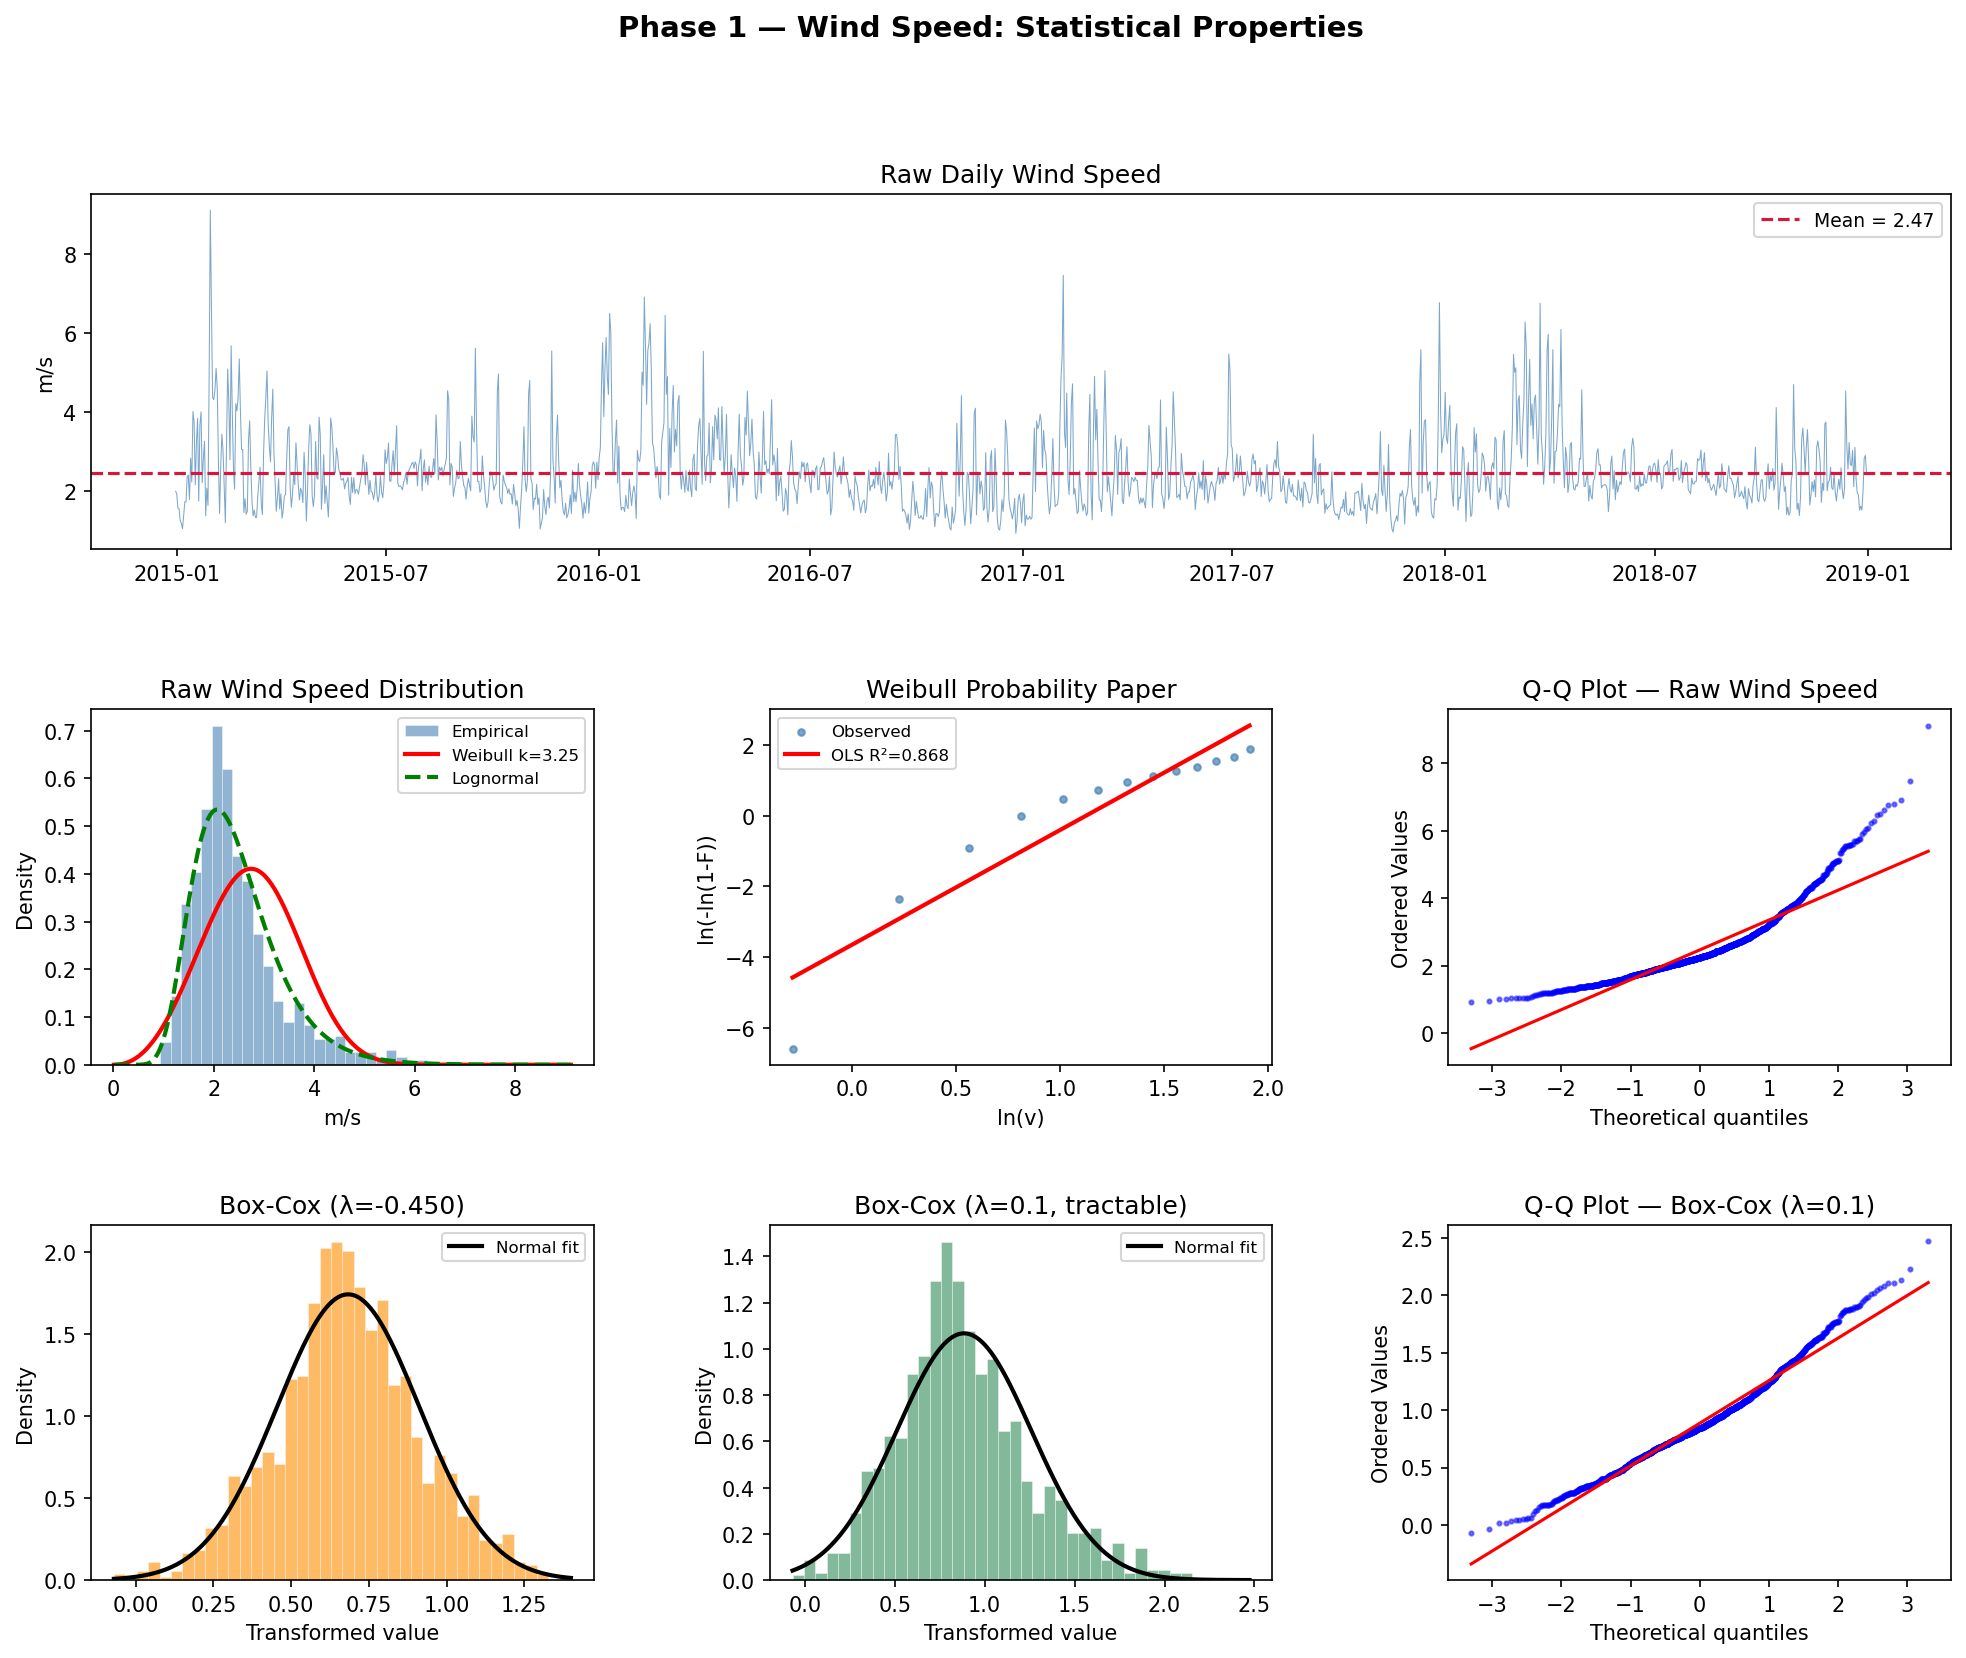
\includegraphics[width=\textwidth]{figures/phase1_wind_analysis.png}
\caption{Dataset A}
\end{subfigure}
\hfill
\begin{subfigure}{0.48\textwidth}
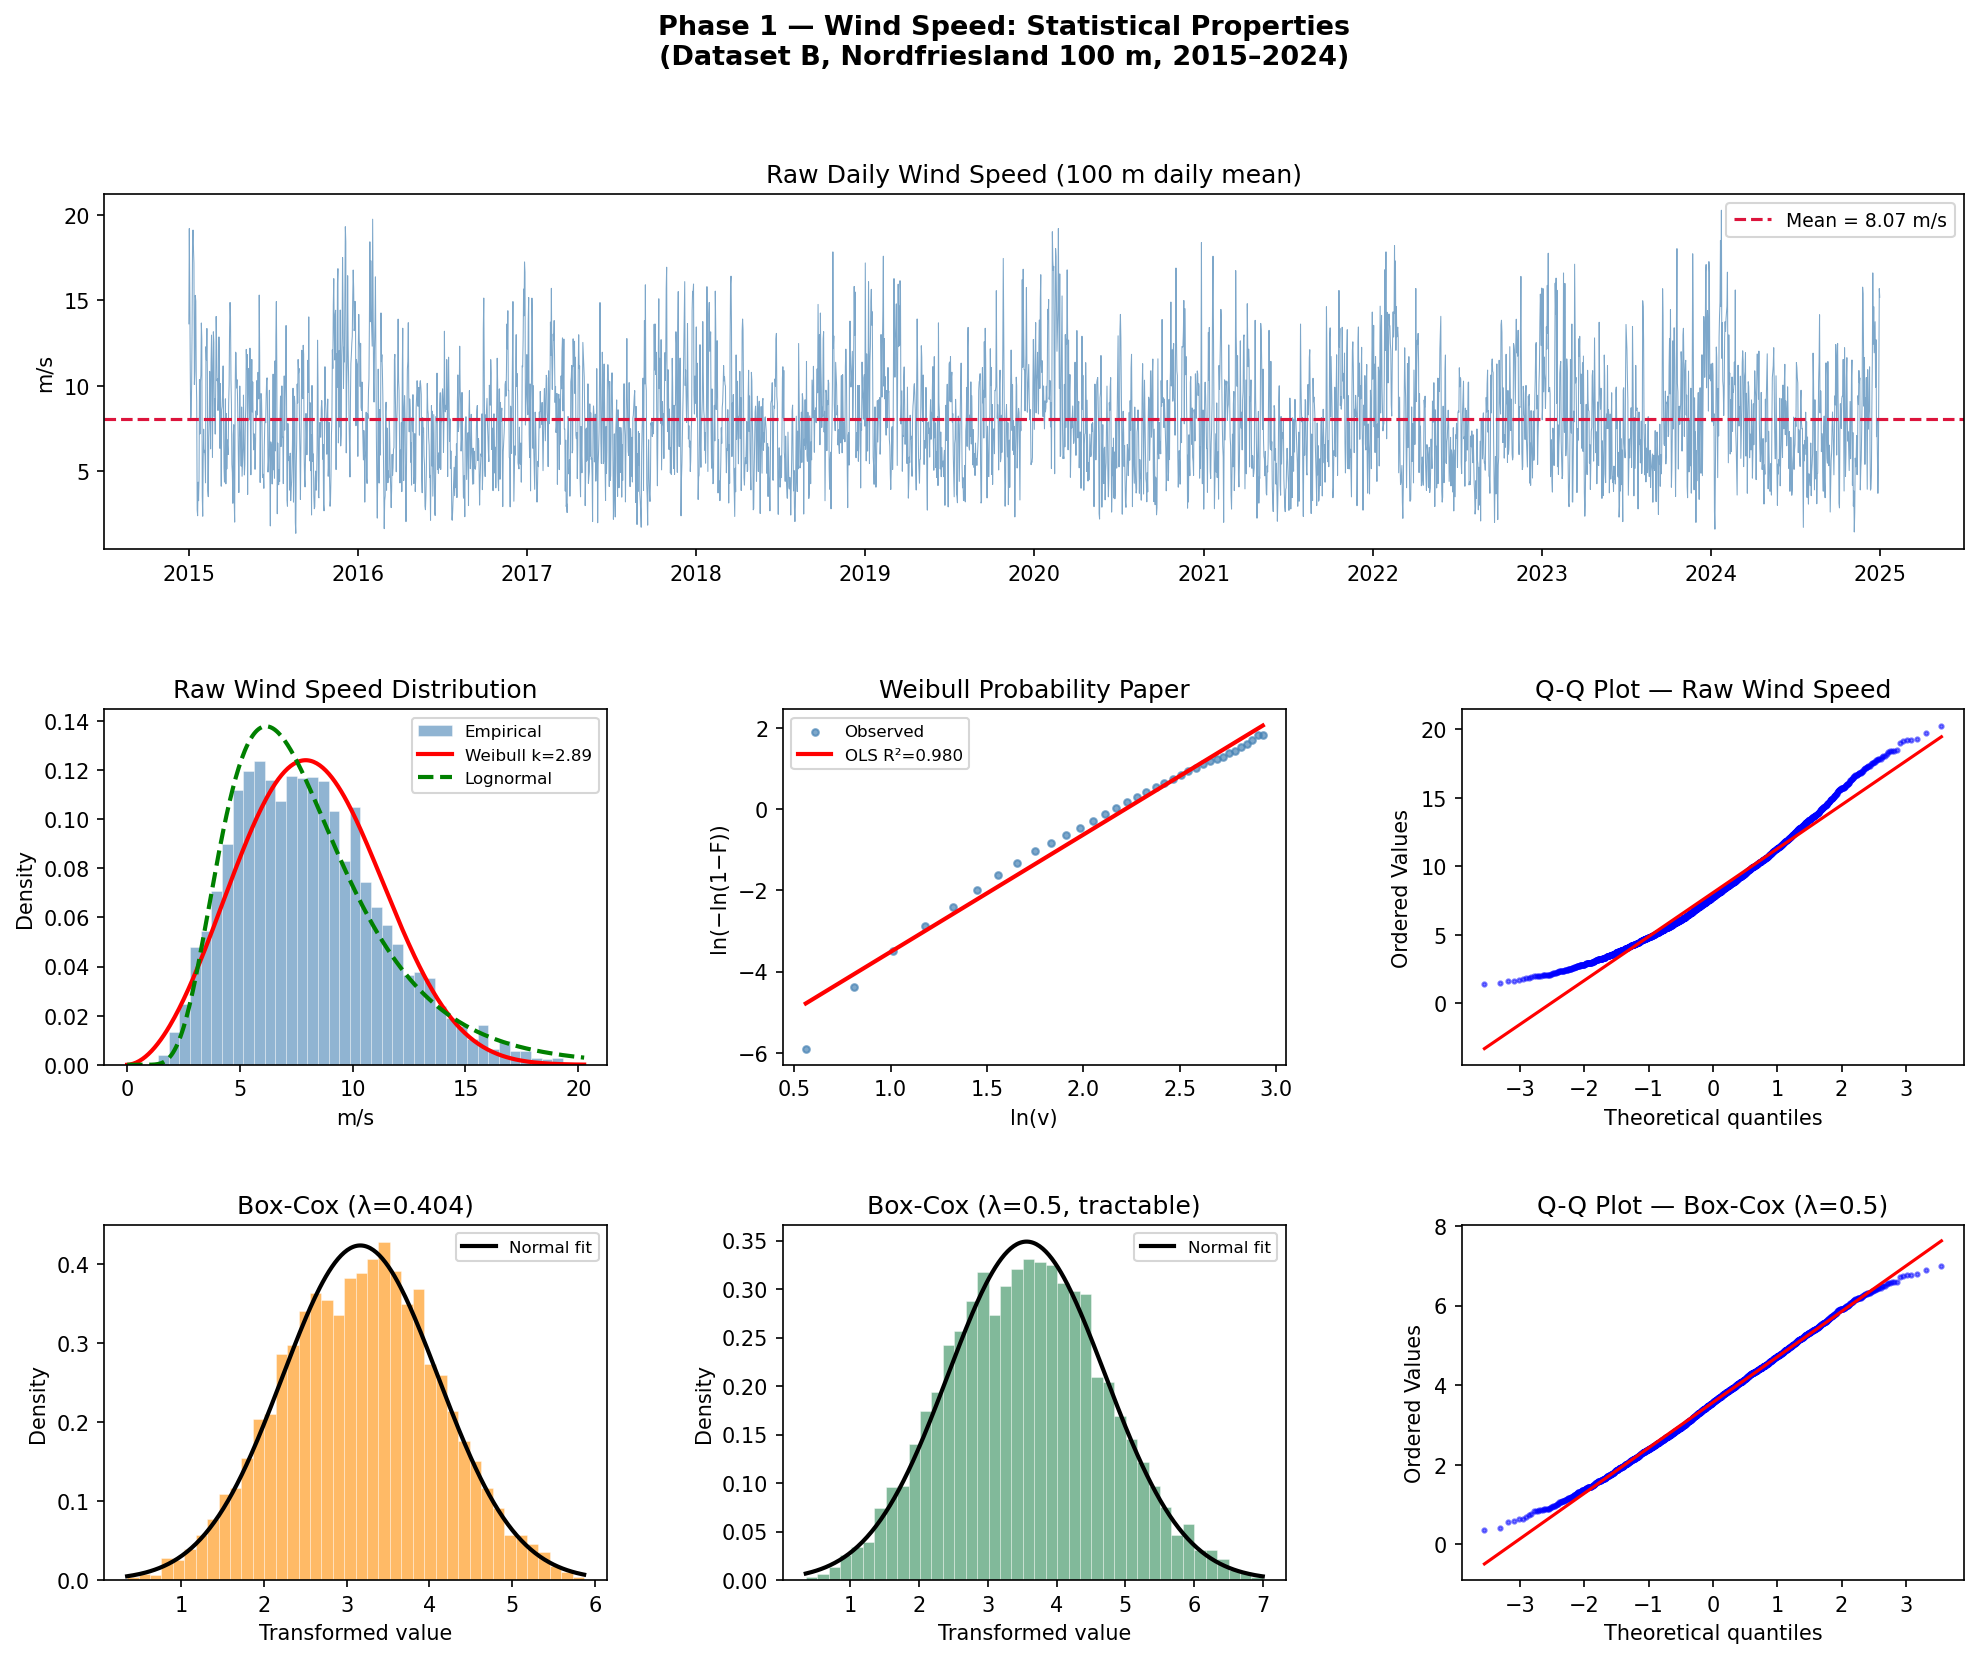
\includegraphics[width=\textwidth]{figures/phase1_B_wind_analysis.png}
\caption{Dataset B}
\end{subfigure}
\caption{Raw wind speed distribution and Box--Cox transformation, both datasets. Each panel is arranged in four rows, read top to bottom. \textbf{Row 1:} the raw daily wind speed time series, with the sample mean marked by a dashed line. \textbf{Row 2:} three diagnostics for the raw series -- a histogram with the fitted Weibull and lognormal densities overlaid, a Weibull probability-paper linearisation, and a quantile--quantile plot against the normal distribution, which shows the characteristic S-curve deviation of a right-skewed, heavy-tailed series. \textbf{Row 3:} histogram and quantile--quantile plot of the series after the likelihood-optimal Box--Cox transformation $\lambda_{\text{opt}}$. \textbf{Row 4:} histogram and quantile--quantile plot after the tractable Box--Cox value actually adopted ($\lambda = 0.1$ for Dataset A, $\lambda = 0.5$ for Dataset B), showing the residual departure from normality left by the tractability constraint discussed in Section~\ref{sec:phase1-boxcox}.}
\label{fig:phase1-wind}
\end{figure}

\subsection{Box--Cox Transformation}
\label{sec:phase1-boxcox}

The Box--Cox family $W^{(\lambda)}(t) = [W(t)^\lambda - 1]/\lambda$ (with $\ln W(t)$ for $\lambda = 0$) is fitted by maximising the profile log-likelihood under a normality assumption. For Dataset A, the likelihood-maximising value is $\lambda_{\text{opt}} = -0.450$, achieving near-perfect Gaussianisation (skewness $-0.005$, excess kurtosis $+0.128$, Jarque--Bera $p = 0.606$). For Dataset B, the optimum is $\lambda_{\text{opt}} = 0.404$, a much less extreme transformation, consistent with the higher hub-height mean wind speed producing a less severely skewed raw distribution. In both cases, the pricing formulas developed in Section~\ref{sec:phase4} and used throughout Chapter~3 require $1/\lambda$ to be a positive integer, so the likelihood optimum cannot be used directly. The requirement that $1/\lambda \in \mathbb{Z}^+$ is dictated by the analytical pricing formulas of Chapter~3. Pricing a forward contract requires computing the expected future wind speed in its original physical measure. Inverting the Box--Cox transformation requires taking the $(1/\lambda)$-th moment of a normal random variable, denoted $M_{1/\lambda}$ \citep{BenthSaltyteBenth2009}. If $1/\lambda$ were fractional, this expectation would lack a closed-form solution and risk generating complex numbers from negative intermediate states, destroying the model's analytical tractability. Following \citet{BenthSaltyteBenth2009}, who adopt $\lambda \in \{0.1, 0.2\}$ for the same CAR$(p)$ continuous-time embedding, $\lambda = 0.1$ is adopted for Dataset A and $\lambda = 0.5$ for Dataset B (Table~\ref{tab:boxcox}). The rounding cost is asymmetric: Dataset A's tractable value sits 0.35 units from its optimum and leaves a residual right skew (skewness $0.601$, Jarque--Bera $p \approx 0$), while Dataset B's tractable value sits only 0.10 units from its optimum and retains near-Gaussian shape (skewness $0.081$, KS $p = 0.091$).

\begin{table}[htbp]
\centering
\caption{Box--Cox transformation: optimal versus tractable $\lambda$.}
\label{tab:boxcox}
\begin{tabular}{l l l}
\toprule
& \textbf{Dataset A} & \textbf{Dataset B} \\
\midrule
$\lambda_{\text{opt}}$ (likelihood-maximising) & $-0.450$ & $0.404$ \\
Gaussianisation at $\lambda_{\text{opt}}$ (skew, JB $p$) & $-0.005$, $0.606$ & $-0.020$, $0.0002$ \\
$\lambda$ adopted (tractable, $1/\lambda \in \mathbb{Z}^+$) & $\mathbf{0.1}$ ($1/\lambda = 10$) & $\mathbf{0.5}$ ($1/\lambda = 2$) \\
Residual shape at adopted $\lambda$ (skew, JB $p$) & $0.601$, $\approx 0$ & $0.081$, $< 0.001$ \\
\bottomrule
\end{tabular}
\end{table}

\subsection{Seasonal Mean and Seasonal Variance}
\label{sec:phase1-seasonal}

Both the seasonal mean $\Lambda(t)$ and the seasonal variance $\sigma^2(t)$ are fitted as two-harmonic truncated Fourier series in calendar day-of-year, $\Lambda(t) = a_0 + \sum_{k=1}^2 [a_k \cos(2\pi k t/365) + b_k \sin(2\pi k t /365)]$ by ordinary least squares, and $\sigma^2(t) = c_0 + \sum_{k=1}^2 c_k \cos(2\pi k t/365)$ (cosine-only, reflecting the approximate symmetry of the variance cycle about its annual peak) fitted to the per-calendar-day empirical variance of the residuals $\varepsilon(t) = W^{(\lambda)}(t) - \Lambda(t)$. Table~\ref{tab:seasonal} reports both fits. The annual harmonic dominates the seasonal mean in both datasets ($b_1$ significant, $a_1$ not, for Dataset A; $a_1$ significant, $b_2$ not, for Dataset B), and the fitted $R^2$ is modest in both cases (0.126 and 0.103): most of the variance in daily wind speed is weather-driven, not calendar-driven, a finding consistent across both the four-year proxy sample and the ten-year reference sample. The seasonal-variance fit is more informative for the purposes of this thesis, since its intercept $C_0$ is the Fourier constant that enters the variance-swap pricing formula $K_{\text{var}}^B = h \times C_0$ used throughout Chapter~3: $C_0 = 0.13138$ for Dataset A versus $C_0 \approx 1.163$ for Dataset B, an 8.8-fold gap that Chapter~3's Value-of-Information analysis identifies as the dominant driver of the pricing error attributable to using the geographic proxy. Both datasets place peak seasonal variance in winter, though the relative modulation differs sharply: Dataset A's fitted $\sigma^2(t)$ ranges over $[0.032, 0.224]$, a winter-to-summer ratio of approximately $6.9$ to $1$, versus Dataset B's much milder range of $[0.944, 1.463]$, a ratio of approximately $1.55$ to $1$.

\begin{table}[htbp]
\centering
\small
\caption{Seasonal mean and seasonal variance Fourier fits, both datasets.}
\label{tab:seasonal}
\begin{tabular}{l l l}
\toprule
& \textbf{Dataset A} & \textbf{Dataset B} \\
\midrule
\multicolumn{3}{l}{\textit{Seasonal mean $\Lambda(t)$}} \\
$a_0$ & $0.88513$ (***) & $3.564$ (***) \\
$a_1$ (annual cos) & $-0.00544$ (n.s.) & $0.510$ (***) \\
$b_1$ (annual sin) & $0.16381$ (***) & $0.083$ (**) \\
$R^2$ & $0.126$ & $0.103$ \\
\midrule
\multicolumn{3}{l}{\textit{Seasonal variance $\sigma^2(t)$}} \\
$C_0$ (mean level) & $0.13138$ (***) & $1.16277$ (***) \\
$c_1$ (annual cos) & $0.09579$ (***) & $0.25933$ (***) \\
$c_2$ (semi-annual cos) & $-0.00332$ (n.s.) & $0.04077$ (n.s.) \\
$R^2$ & $0.226$ & $0.116$ \\
$\sigma^2(t)$ range & $[0.032, 0.224]$ & $[0.944, 1.463]$ \\
\bottomrule
\end{tabular}
\end{table}

\subsection{The Standardised Series $\widetilde W(t)$}
\label{sec:phase1-wtilde}

The standardised series $\widetilde W(t) = \varepsilon(t)/\sigma(t)$ is, by construction, close to zero-mean and unit-variance in both datasets (Dataset A: mean $0.001$, std.\ $0.967$; Dataset B: mean $-0.00003$, std.\ $1.005$), confirming that the centring and scaling steps were executed correctly. Neither series is yet white noise, however. The Ljung--Box statistic tests the joint null hypothesis that the first $m$ autocorrelations of a series are zero,
\begin{equation}
LBQ(m) = n(n+2)\sum_{k=1}^m \frac{\hat\rho(k)^2}{n-k} \ \sim\ \chi^2(m) \quad \text{under } H_0,
\end{equation}
where $\hat\rho(k)$ is the sample autocorrelation at lag $k$; applied to a series' squared values, the same statistic tests for conditional heteroskedasticity rather than serial correlation in levels. The test rejects the null of no serial correlation at every tested lag (5, 10, 20) for $\widetilde W(t)$ itself in both datasets ($p < 0.001$), and the same test applied to $\widetilde W(t)^2$ also rejects at every lag in both datasets ($p < 0.001$), indicating conditional heteroskedasticity beyond the deterministic seasonal variance already removed. These two findings are the direct motivation for the AR(4) mean model of Section~\ref{sec:phase2} and the GARCH(1,1) volatility model of Section~\ref{sec:phase3} respectively, and the pattern is identical across both datasets despite their very different sample lengths and measurement heights. This is evidence that the residual dynamics being modelled are a genuine feature of daily wind speed, not an artefact of one particular site or sample.

\begin{figure}[htbp]
\centering
\begin{subfigure}{0.48\textwidth}
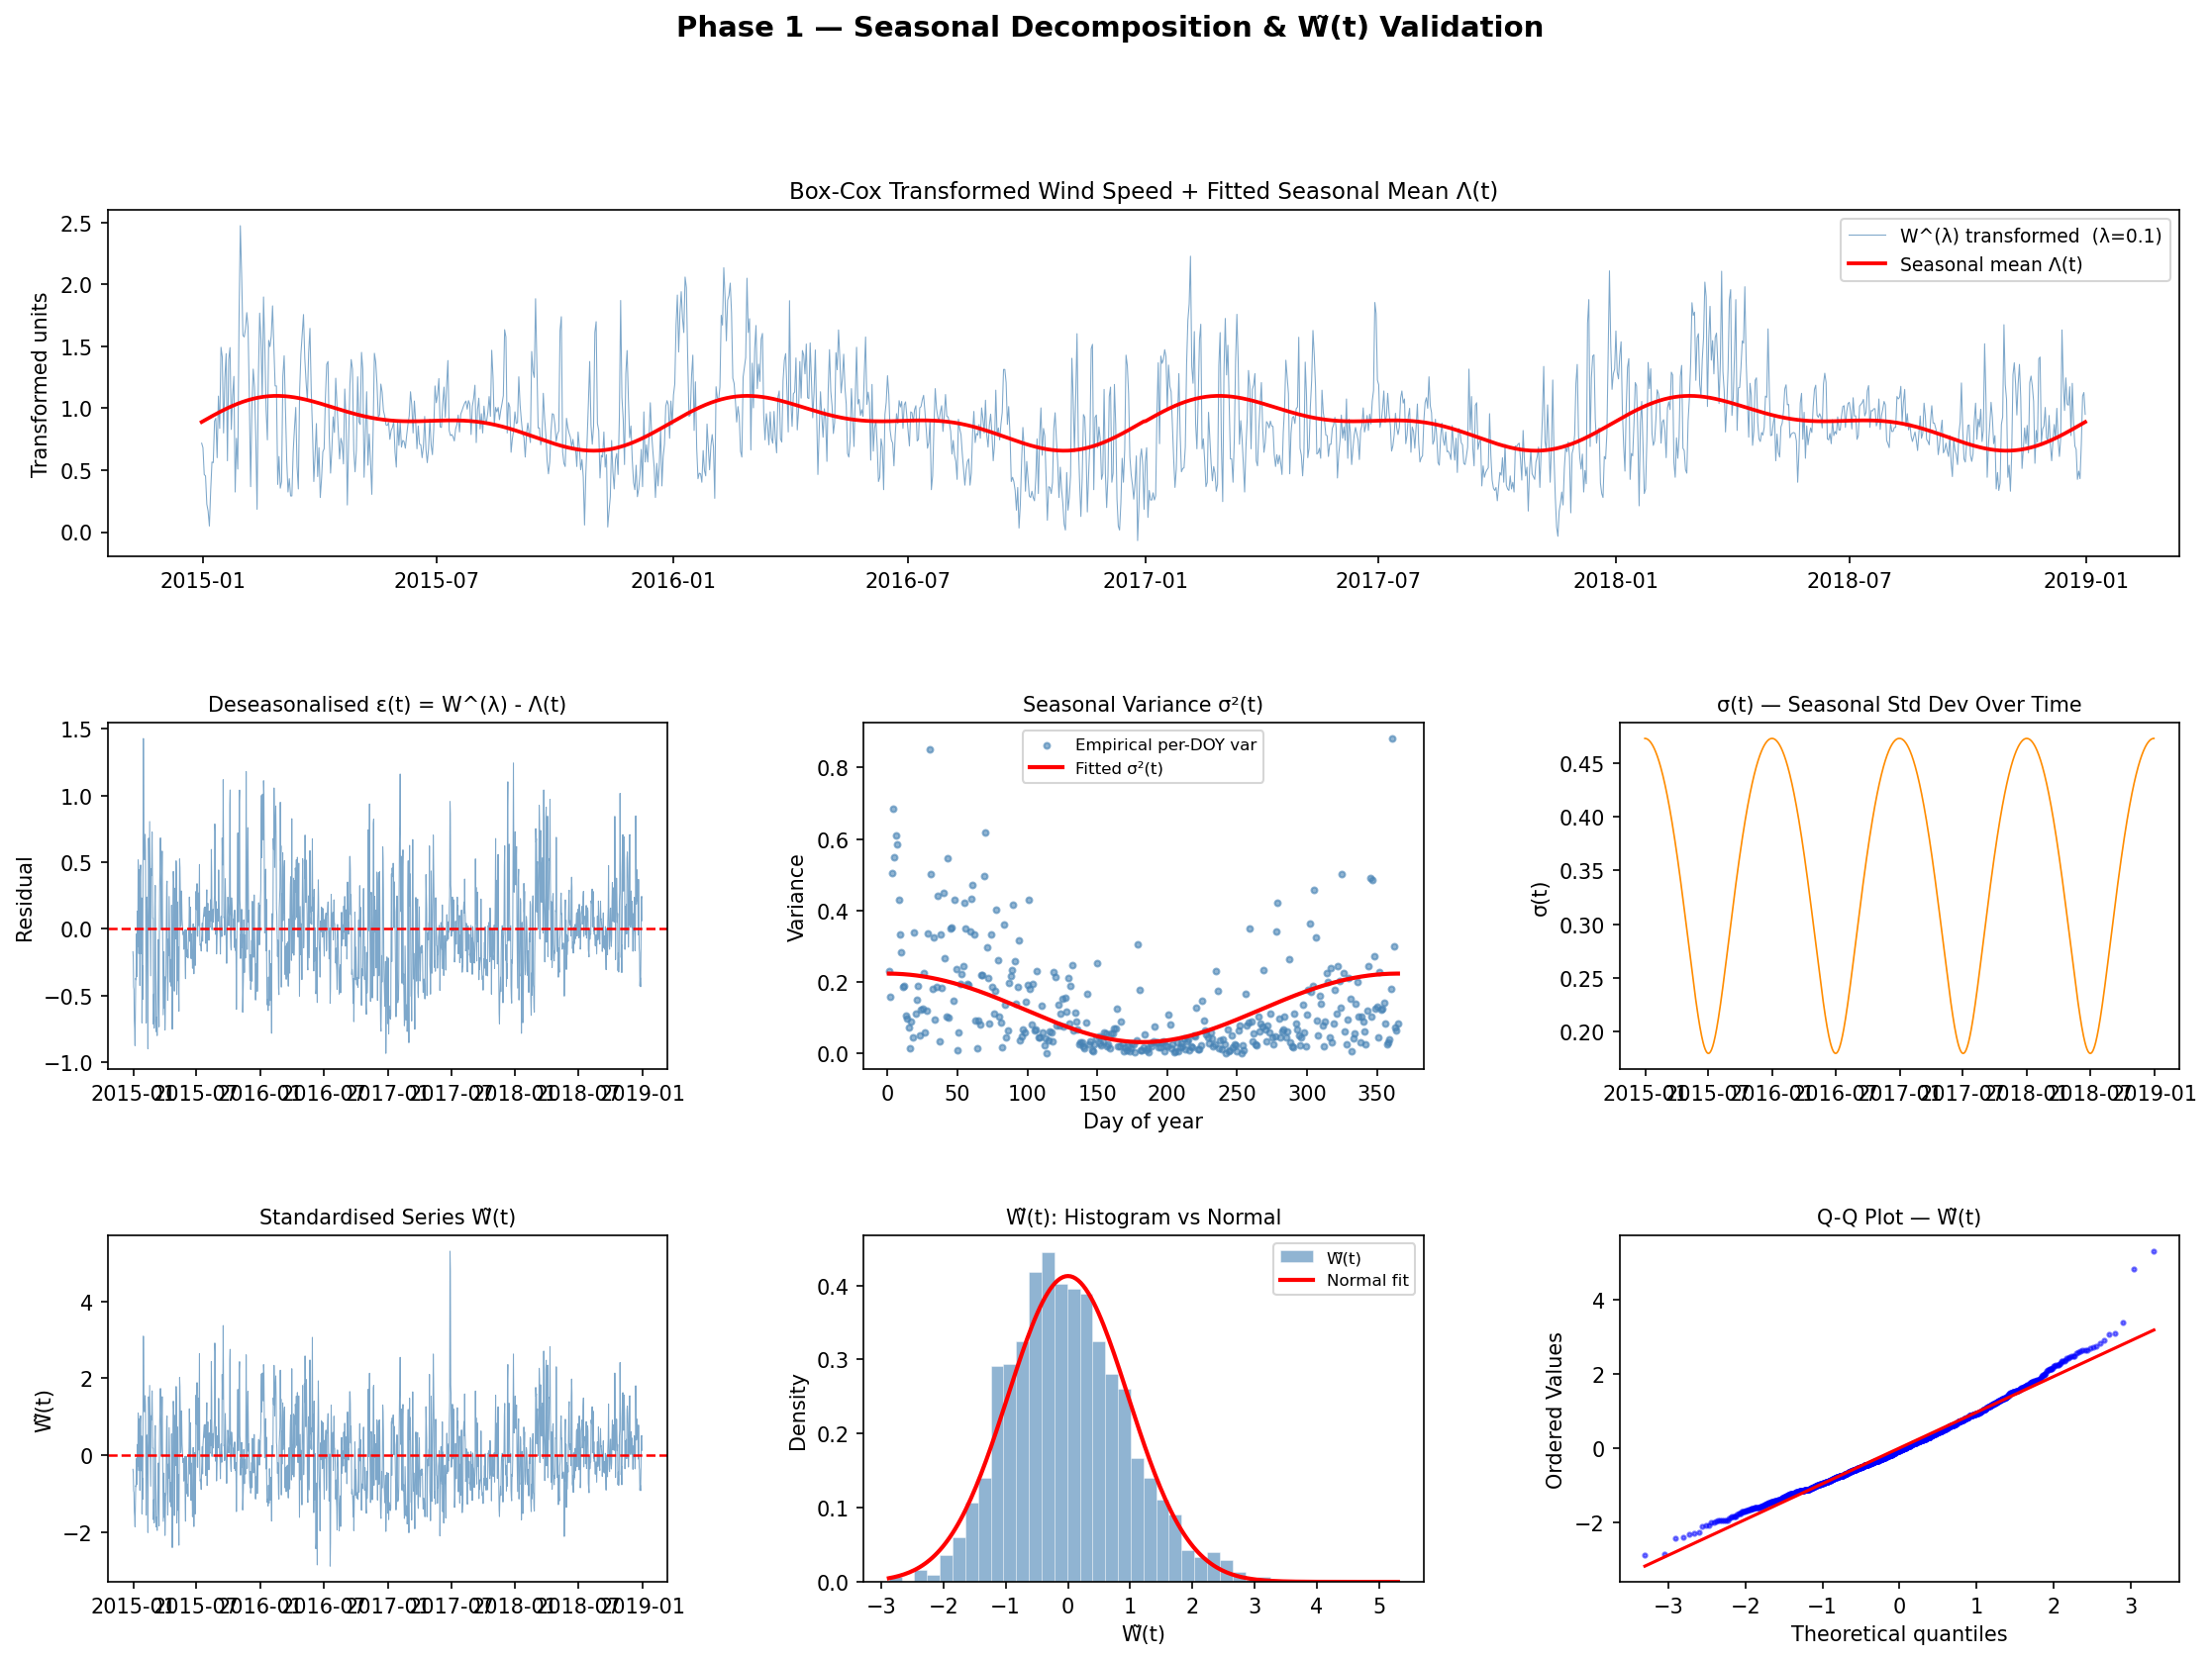
\includegraphics[width=\textwidth]{figures/phase1_seasonal_decomposition.png}
\caption{Dataset A}
\end{subfigure}
\hfill
\begin{subfigure}{0.48\textwidth}
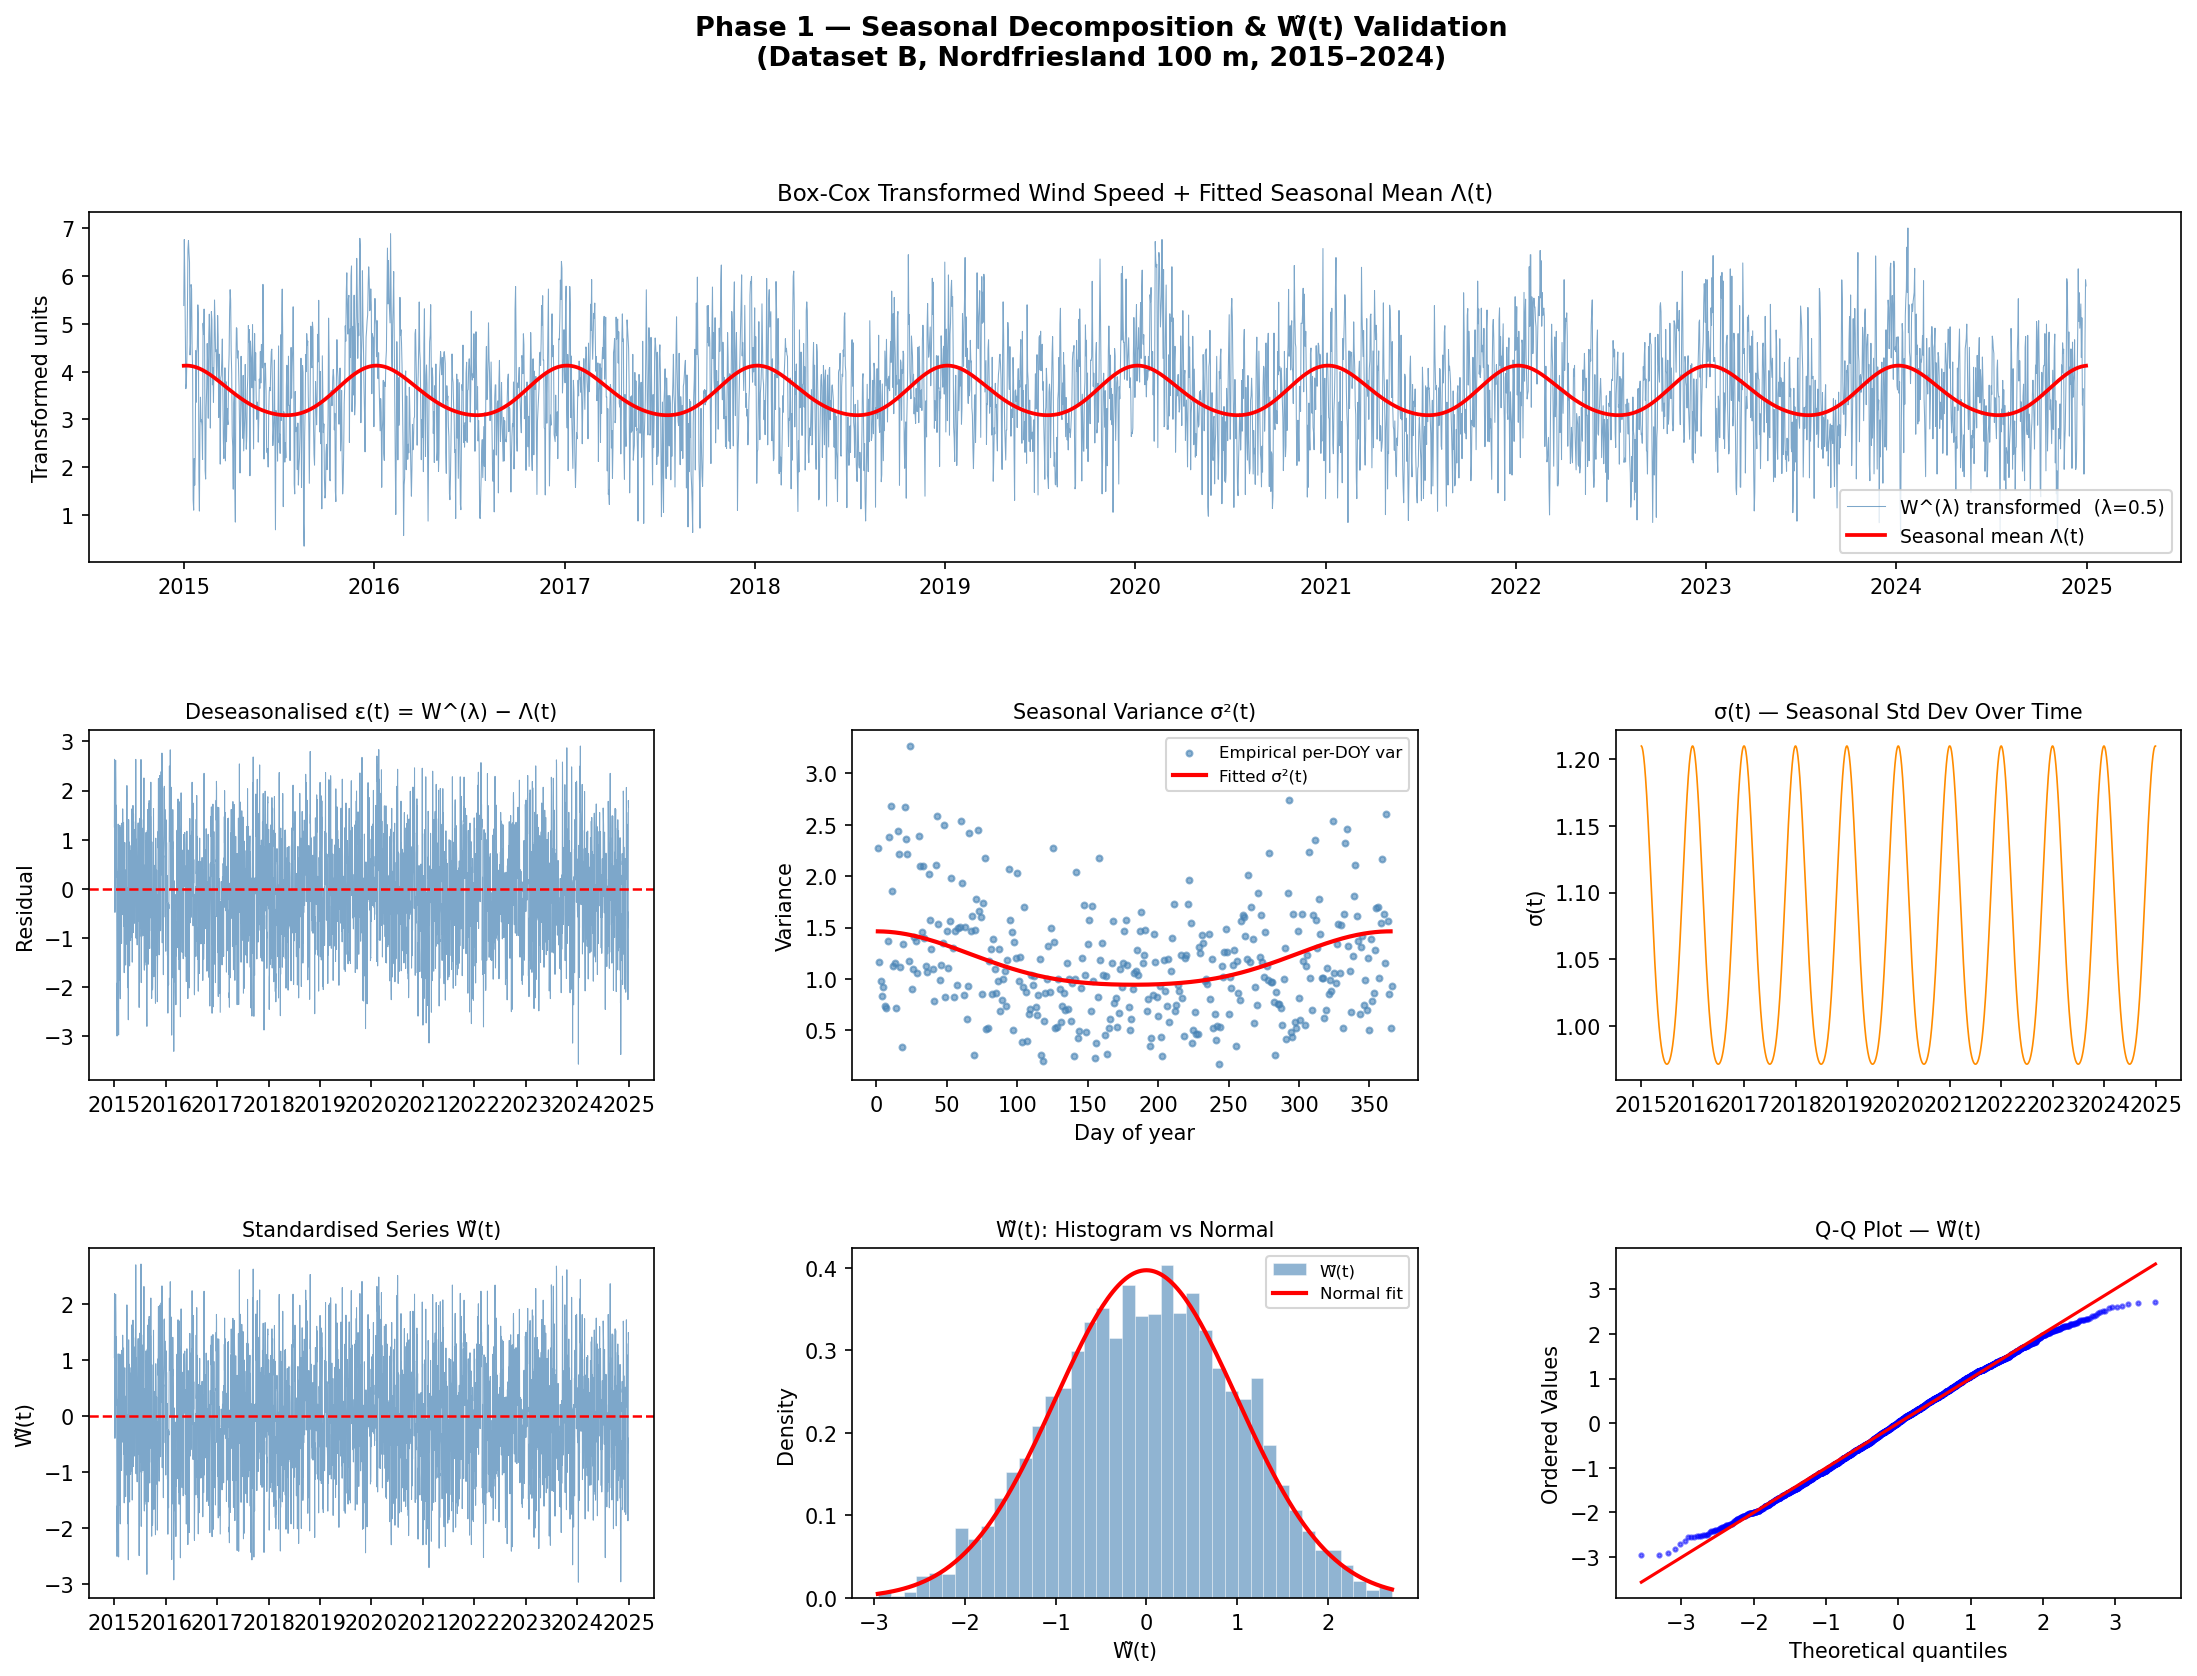
\includegraphics[width=\textwidth]{figures/phase1_B_seasonal_decomposition.png}
\caption{Dataset B}
\end{subfigure}
\caption{Seasonal decomposition and standardisation, both datasets. Each panel is arranged in three rows. \textbf{Row 1:} the transformed wind speed $W^{(\lambda)}(t)$ with the fitted seasonal mean $\Lambda(t)$ overlaid. \textbf{Row 2:} three panels -- the deseasonalised residuals $\varepsilon(t) = W^{(\lambda)}(t) - \Lambda(t)$; the empirical per-calendar-day variance (points) with the fitted Fourier seasonal-variance curve $\sigma^2(t)$ (line), showing the winter peak / summer trough pattern common to both datasets; and, third, an autocorrelation plot of the seasonal standard deviation curve across the calendar year, a supplementary panel not otherwise discussed in the main text. \textbf{Row 3:} the standardised series $\widetilde W(t)$, its histogram against a normal density, and a quantile--quantile plot, illustrating the residual serial dependence and non-normality quantified in Section~\ref{sec:phase1-wtilde}.}
\label{fig:phase1-seasonal}
\end{figure}

\section{Conditional Mean: AR(4)}
\label{sec:phase2}

The Ljung--Box evidence of Section~\ref{sec:phase1-wtilde} establishes that $\widetilde W(t)$ retains serial dependence. This section fits an autoregressive model to capture it.

\subsection{Order Selection}
\label{sec:phase2-order}

Both datasets exhibit a similar autocorrelation profile: a partial autocorrelation function (PACF) with clearly significant spikes at lags 1--3 and a markedly weaker, borderline value at lag 4 (Dataset A: PACF$_4 = 0.0311$, just inside the 95\% band; Dataset B: PACF$_4 = -0.0070$, effectively zero), with no significant structure beyond lag~4 in either series. An AIC/BIC grid search over AR($p$), $p = 1,\dots,6$, in fact selects AR(3) as the minimum-AIC model for \emph{both} datasets (Dataset A: AIC $= 3{,}432.24$ at $p=3$ versus $3{,}432.83$ at $p=4$, a difference of 0.59 units; Dataset B: AIC $=9{,}342.24$ at $p=3$ versus $9{,}344.04$ at $p=4$, a difference of 1.8 units), and in both cases the gap falls within the conventional two-point AIC band below which two models are considered statistically indistinguishable.

AR(4) is nonetheless retained as the operating specification in both datasets, on structural rather than statistical grounds: the continuous-time CAR(4) embedding of Section~\ref{sec:phase4} requires a companion matrix of dimension four, and the Euler-discretisation mapping from discrete AR coefficients $\{\beta_1,\dots,\beta_4\}$ to continuous CAR coefficients $\{\alpha_1,\dots,\alpha_4\}$, following \citet{BenthSaltyteBenth2009}, does not generalise to a three-lag or mixed ARMA specification. This is a deliberate trade-off, stated candidly here rather than left implicit: a fractionally-smaller-AIC three-lag model is set aside in favour of the four-lag model that the pricing framework of Chapter~3 actually requires, on the grounds that the statistical cost of doing so is, in both datasets, within the range normally treated as noise.

\subsection{AR(4) Coefficients}
\label{sec:phase2-coefs}

Table~\ref{tab:ar4} reports the fitted AR(4) coefficients for both datasets, estimated on the zero-mean series $\widetilde W(t)$ without an intercept. Both datasets show the coefficient magnitude declining with lag order and a positive, dominant $\beta_1$, but the two series differ in the sign of $\beta_4$ (Dataset A: $+0.0310$; Dataset B: $-0.0074$) and in the statistical significance of the higher lags: Dataset A's $\beta_2$ and $\beta_3$ are both significant at the 1\% level and $\beta_4$ is not significant ($p = 0.208$), while Dataset B's $\beta_3$ is only marginally significant ($p = 0.090$) and $\beta_4$ is clearly insignificant ($p = 0.660$). Neither discrepancy affects the modelling decision, since AR(4) is retained structurally regardless of the marginal significance of its highest lag, but both are reported here rather than smoothed over, since a coefficient that changes sign between the two datasets is a legitimate empirical finding, not a data-quality concern.

\begin{table}[htbp]
\centering
\caption{AR(4) coefficients, both datasets (OLS/MLE on $\widetilde W(t)$, no intercept).}
\label{tab:ar4}
\begin{tabular}{l r r r r}
\toprule
& \multicolumn{2}{c}{\textbf{Dataset A}} & \multicolumn{2}{c}{\textbf{Dataset B}} \\
\textbf{Coefficient} & \textbf{Estimate} & \textbf{$p$-value} & \textbf{Estimate} & \textbf{$p$-value} \\
\midrule
$\beta_1$ & $0.6299$ & $<0.001$ & $0.5324$ & $<0.001$ \\
$\beta_2$ & $-0.1443$ & $<0.001$ & $-0.0763$ & $<0.001$ \\
$\beta_3$ & $0.0926$ & $0.001$ & $0.0324$ & $0.090$ \\
$\beta_4$ & $0.0310$ & $0.208$ & $-0.0074$ & $0.660$ \\
\bottomrule
\end{tabular}
\end{table}

Both coefficient sets can be read against the New York daily wind-speed AR(4) fit reported by \citet{AlexandridisZapranis2013}: $\beta_1=0.362$, $\beta_2=-0.100$, $\beta_3=0.027$, $\beta_4=0.022$. Dataset A's coefficients are larger in magnitude than the New York benchmark at every lag. Dataset B's are larger at $\beta_1$ ($0.532$ versus $0.362$) and $\beta_3$ ($0.032$ versus $0.027$), but smaller at $\beta_2$ ($0.076$ versus $0.100$ in magnitude) and $\beta_4$ ($0.007$ versus $0.022$), so the comparison holds cleanly for the proxy dataset but only partially for the reference dataset. The dominant lag-1 coefficient, which carries most of the autoregressive structure in both series, is larger at both European sites than at the New York site, and this is attributed, in the underlying phase analysis, to a stronger lag-1 sample autocorrelation at both European sites (0.579 for Dataset A) than at the New York site ($\approx 0.36$), consistent with the sites' differing synoptic exposure rather than with any difference in modelling approach: the AR(4) specification itself is identical to the one used in the benchmark study.

For Dataset A, the characteristic roots of the fitted AR(4) polynomial have moduli $\{0.702, 0.470, 0.470, 0.200\}$, all inside the unit circle, confirming stationarity; the dominant root implies a mean-reversion half-life for the level of wind-speed anomalies of approximately 2.0 days. This is a materially faster reversion than the volatility half-life derived from the GARCH model in Section~\ref{sec:phase3} (41.6 and 38.3 days for Datasets A and B respectively): the \emph{level} of a wind-speed anomaly washes out within days, while the \emph{volatility regime} it occurred in persists for weeks, a distinction that recurs when the two dynamics are combined in Section~\ref{sec:phase4}.

\subsection{Residual Diagnostics}
\label{sec:phase2-diag}

Table~\ref{tab:ar4-diag} summarises the Ljung--Box tests on the AR(4) residuals $\hat\varepsilon(t)$ and on their squares. In both datasets, the serial-correlation test on levels passes comfortably at every lag ($p > 0.5$ throughout), confirming that AR(4) has removed the linear dependence identified in Section~\ref{sec:phase1-wtilde}. In both datasets, the test on squared residuals rejects the null of no remaining structure at conventional significance. This is corroborated by the Engle \citeyearpar{Engle1982} Lagrange-multiplier test for autoregressive conditional heteroskedasticity, which regresses squared residuals on their own lags, $\hat\varepsilon(t)^2 = \gamma_0 + \sum_{k=1}^q \gamma_k \hat\varepsilon(t-k)^2 + u(t)$, and tests the joint significance of $\gamma_1,\dots,\gamma_q$ via $\text{LM}(q) = nR^2 \sim \chi^2(q)$ under the null of no ARCH effects; the entry-residual ARCH-LM test is significant in both datasets (Dataset A: $\text{LM}(5) = 18.80$, $p = 0.0021$; Dataset B: $\text{LM}(5) = 16.58$, $p = 0.0054$). This is the expected and desired outcome at this stage: the AR(4) mean equation is adequate, and the conditional heteroskedasticity that remains is precisely what the GARCH(1,1) layer of Section~\ref{sec:phase3} is designed to capture.

\begin{table}[htbp]
\centering
\caption{AR(4) residual diagnostics, both datasets.}
\label{tab:ar4-diag}
\begin{tabular}{l r r}
\toprule
\textbf{Test} & \textbf{Dataset A} & \textbf{Dataset B} \\
\midrule
Ljung--Box $\hat\varepsilon(t)$, lag 20 ($p$) & $0.506$ & $0.511$ \\
Ljung--Box $\hat\varepsilon(t)^2$, lag 20 ($p$) & $0.0033$ & $0.2724^{\ast}$ \\
ARCH-LM(5) on entry residuals ($p$) & $0.0021$ & $0.0054$ \\
\bottomrule
\end{tabular}
\vspace{2pt}
{\footnotesize $^{\ast}$Dataset B's source analysis is internally inconsistent on its squared-residual diagnostics: the narrative text reports that the Ljung--Box test rejects homoskedasticity at lags 5 and 10 ($p = 0.0048$ and $0.0419$), while the lag-20 value tabulated there is $0.2724$ (a pass). The cell above reports the lag-20 value from the source table. Note that lags 5 and 10 rejections are the substantive finding motivating GARCH, regardless of the lag-20 outcome, and the ARCH-LM entry-residuals test (final row) is independently significant in both datasets.}
\end{table}

\subsection{Forecast Accuracy versus Persistence}
\label{sec:phase2-rmse}

Table~\ref{tab:ar4-rmse} reports one-step-ahead out-of-sample forecast accuracy against a persistence benchmark $\hat{\widetilde W}(t) = \widetilde W(t-1)$, using a walk-forward evaluation held out from the estimation sample. AR(4) reduces RMSE relative to persistence by 12.2\% in Dataset A and 13.8\% in Dataset B, and a Diebold--Mariano test \citep{DieboldMariano1995} rejects the null of equal predictive accuracy in both cases (Dataset A: $DM = -3.681$, $p = 0.0002$; Dataset B: $DM = -7.019$, $p < 0.001$). These are the frozen benchmark figures for the two datasets and are reused, without re-estimation, in the cross-dataset validation exercise of Chapter~3; a separate, later validation split reported there for Dataset B under the same Diebold--Mariano procedure (Section~3.2) uses a different train/test partition and yields a similar but not numerically identical improvement (13.6\%), a difference attributable entirely to the split rather than to any change in the fitted model, and reported explicitly as such where it recurs.

Two features of the Diebold--Mariano statistics themselves should be noted, since the figures quoted here differ from those reported for the same test in Chapter~3. The first is a sign convention. The evaluation used here defines the loss differential as $d_t = e^2_{\text{AR(4)}}(t) - e^2_{\text{persistence}}(t)$, so that a model outperforming the benchmark produces a \emph{negative} statistic; the Chapter~3 evaluation reverses the ordering, differencing the benchmark's squared error first, so the same outcome appears with a positive sign. The two are the same test reaching the same conclusion, and both reject the null at any conventional level. The second is magnitude: the statistics reported there are larger in absolute value ($8.26$ and $16.76$, against $3.681$ and $7.019$ here) because they are computed on the full standardised series rather than on the held-out partition used in this section. A Diebold--Mariano statistic scales with the square root of the evaluation sample, and for Dataset A the ratio of sample sizes alone, $\sqrt{1462/220} \approx 2.6$, accounts for most of the observed ratio of $2.2$.

One further property of the mean model is worth recording here, where the conditional mean is estimated, rather than leaving it to emerge in Chapter~3. The AR(4)+GARCH, CAR(4)+Gaussian and CAR(4)+NIG specifications developed in the following sections all inherit the AR(4) conditional mean unchanged: the GARCH layer of Section~\ref{sec:phase3} models the conditional variance of the residuals, and the CAR(4) embedding of Section~\ref{sec:phase4} is an exact continuous-time representation of the same mean dynamics, so none of the three alters the one-step-ahead point forecast. The four specifications are therefore observationally equivalent at a one-day horizon by construction, and differ only in their conditional-variance and tail representations. This is why the cross-dataset validation of Chapter~3 separates them on pricing and hedging criteria rather than on point-forecast accuracy, where no separation is available in principle.

\begin{table}[htbp]
\centering
\caption{AR(4) vs.\ persistence, one-step-ahead out-of-sample RMSE.}
\label{tab:ar4-rmse}
\begin{tabular}{l r r r r}
\toprule
& \multicolumn{2}{c}{\textbf{Dataset A}} & \multicolumn{2}{c}{\textbf{Dataset B}} \\
& \textbf{RMSE} & \textbf{MAE} & \textbf{RMSE} & \textbf{MAE} \\
\midrule
Persistence & $0.6856$ & $0.5214$ & $0.9955$ & $0.8054$ \\
AR(4) & $0.6017$ & $0.4706$ & $0.8580$ & $0.6950$ \\
Improvement & $12.2\%$ & --- & $13.8\%$ & --- \\
\bottomrule
\end{tabular}
\end{table}

\begin{figure}[htbp]
\centering
\begin{subfigure}{0.48\textwidth}
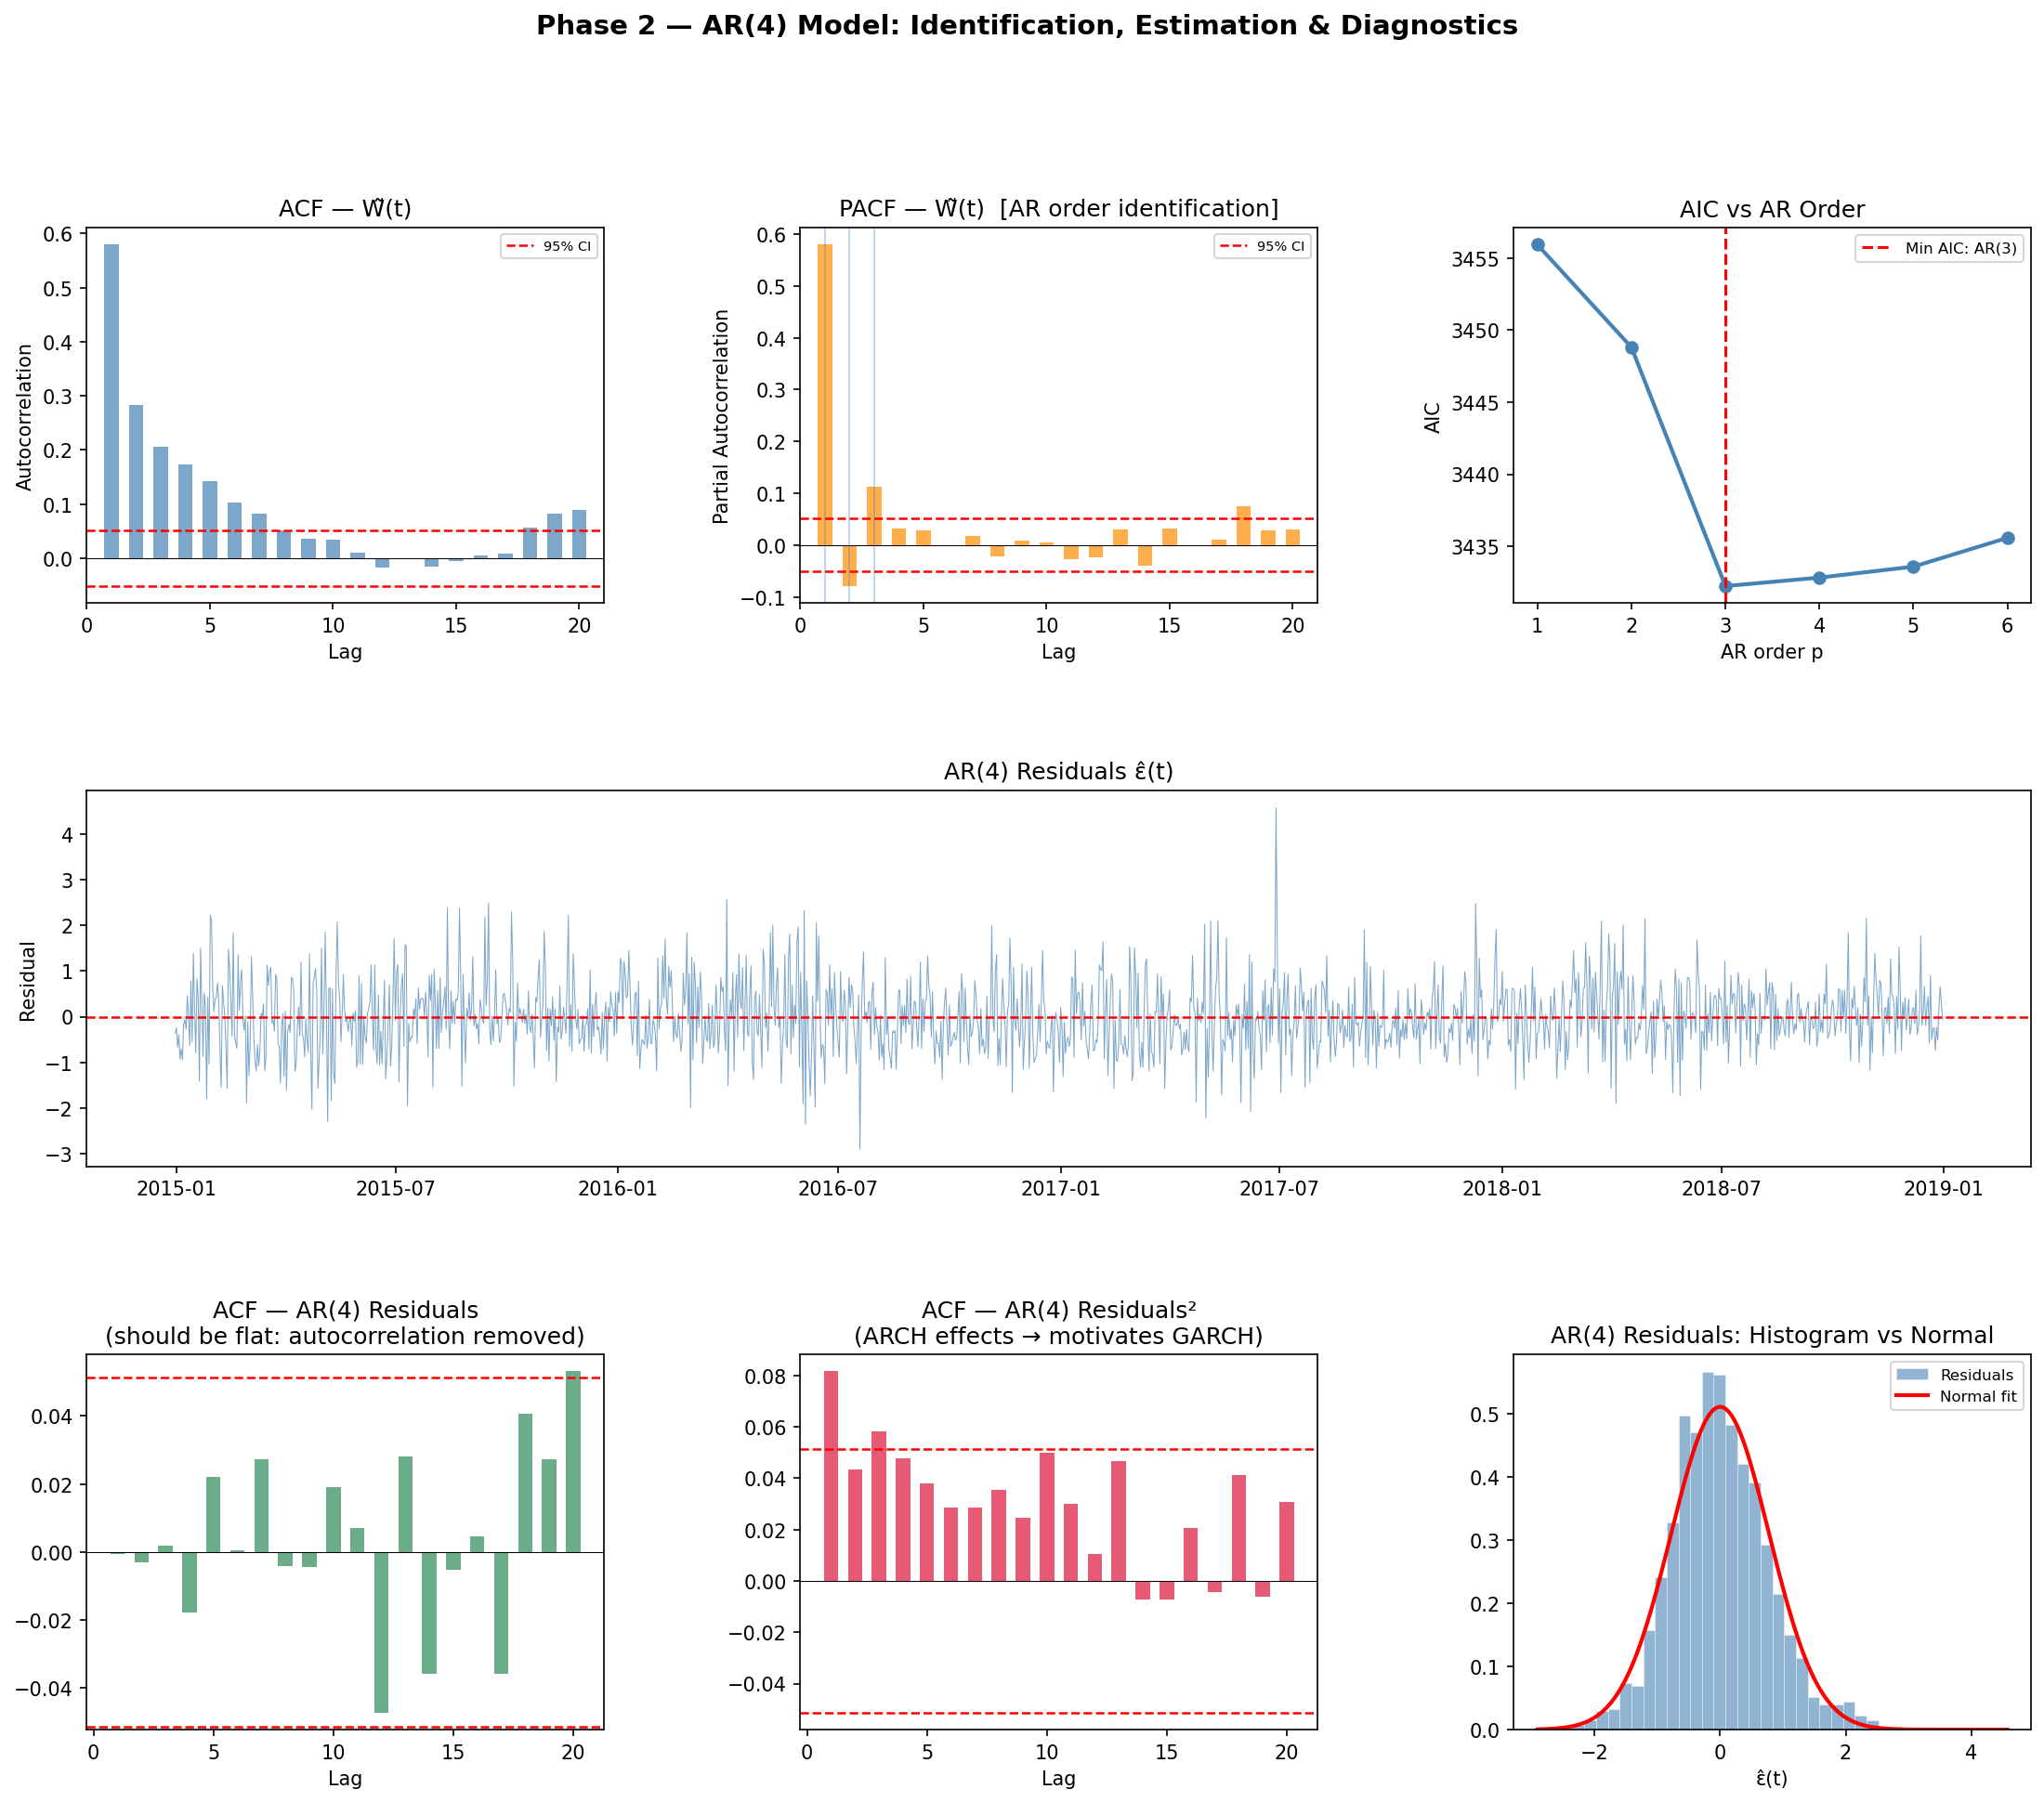
\includegraphics[width=\textwidth]{figures/phase2_ar4_diagnostics.png}
\caption{Dataset A}
\end{subfigure}
\hfill
\begin{subfigure}{0.48\textwidth}
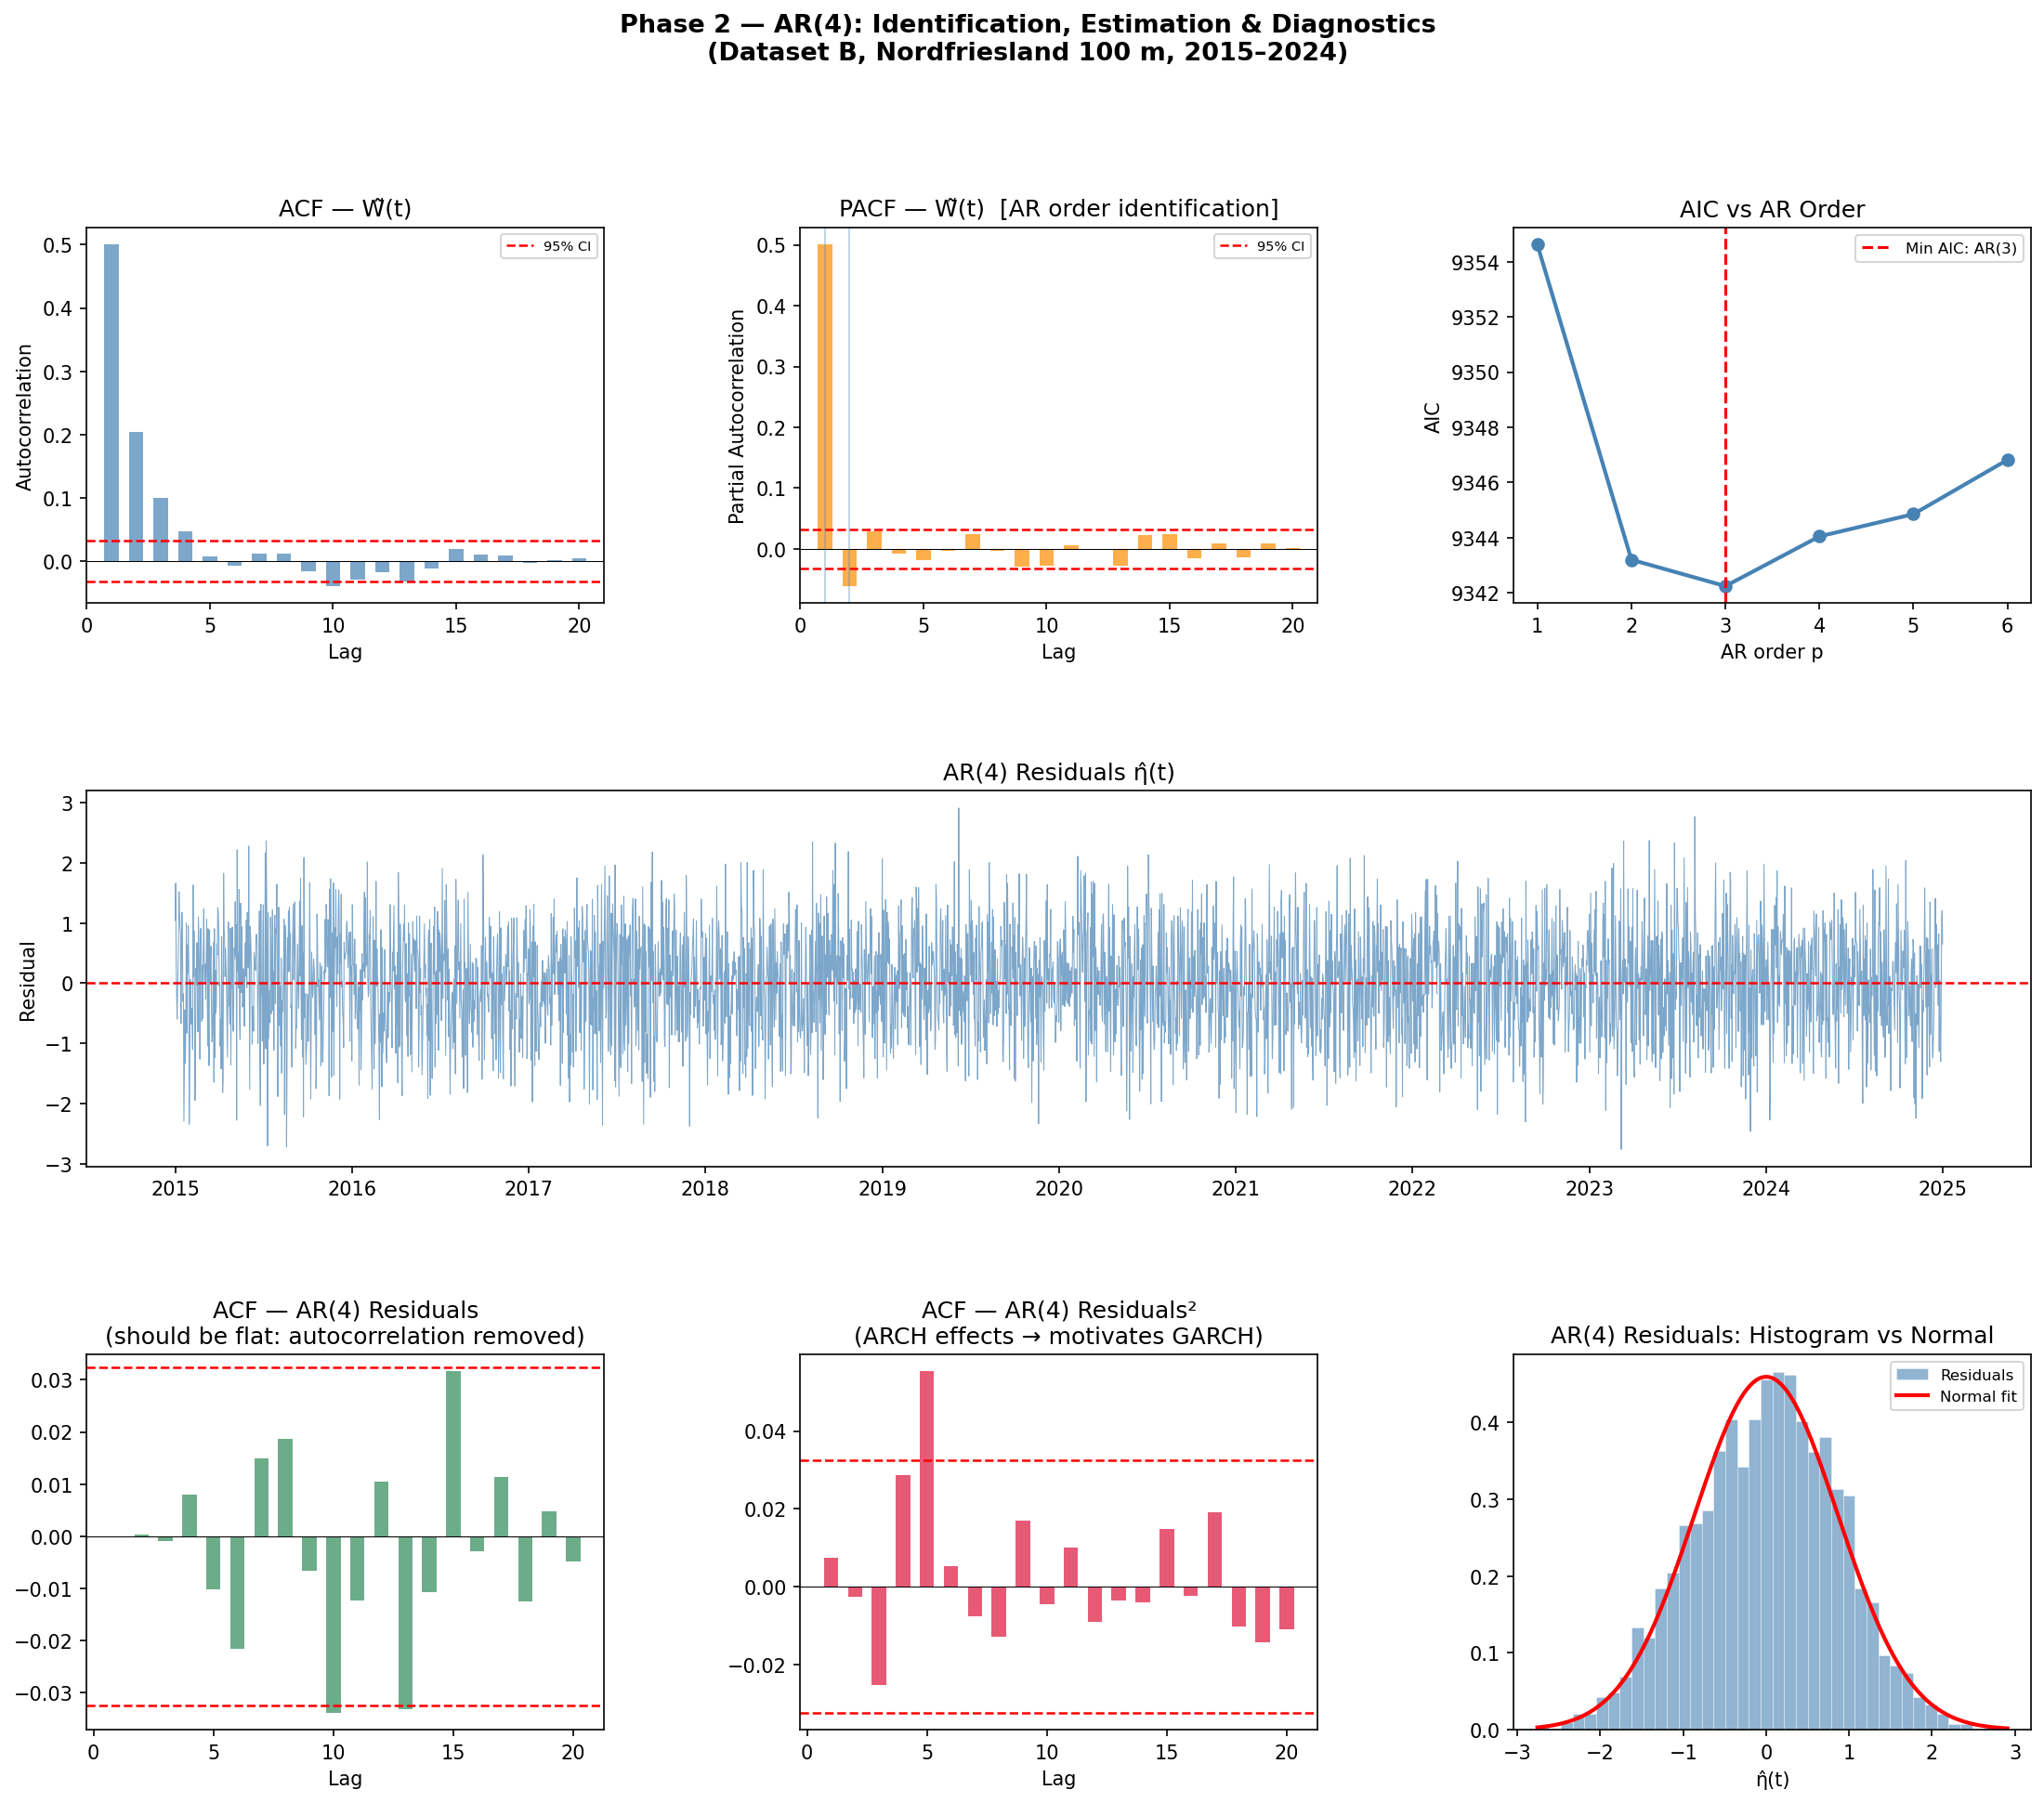
\includegraphics[width=\textwidth]{figures/phase2_B_ar4_diagnostics.png}
\caption{Dataset B}
\end{subfigure}
\caption{AR(4) identification and residual diagnostics, both datasets. Each panel is arranged in three rows. \textbf{Row 1:} three panels -- the autocorrelation function of $\widetilde W(t)$; its partial autocorrelation function, showing the sharp PACF cutoff after lag~4 discussed in Section~\ref{sec:phase2-order}; and the AIC grid search across candidate AR orders. \textbf{Row 2:} the time series of the AR(4) residuals $\hat\varepsilon(t)$. \textbf{Row 3:} three further panels, confirming that AR(4) has removed the linear serial dependence identified in Section~\ref{sec:phase1-wtilde} while conditional heteroskedasticity remains -- an autocorrelation-type diagnostic of $\hat\varepsilon(t)$; the corresponding diagnostic applied to $\hat\varepsilon(t)^2$, which stays visibly elevated and motivates the GARCH model of Section~\ref{sec:phase3}; and a histogram of $\hat\varepsilon(t)$ against a normal density.}
\label{fig:phase2-ar4}
\end{figure}

\subsection{Long Memory}
\label{sec:phase2-longmemory}

A natural question, given the literature reviewed in Section~1.3.2, is whether the residual dependence in $\widetilde W(t)$ decays exponentially, as a finite-order AR model assumes, or hyperbolically, as fractional integration would imply. The Geweke--Porter-Hudak (GPH) log-periodogram estimator regresses the log-periodogram of the series on the log of the frequency, $\ln I(\omega_j) = c - d\ln\left[4\sin^2(\omega_j/2)\right] + u_j$, over the $m = n^{0.6}$ lowest Fourier frequencies $\omega_j$, and tests $H_0: d = 0$ against fractional integration $d \neq 0$. It gives a fractional-differencing parameter of $\hat d = 0.119$ ($p = 0.208$) for Dataset A and $\hat d = -0.115$ ($p = 0.094$) for Dataset B. The interpretation of the two results is not symmetric, and the sign of the second matters. Long memory in the sense at issue here requires $0 < d < 0.5$; a negative $\hat d$ indicates anti-persistence, a hyperbolically decaying but sign-alternating dependence structure that is the opposite of long memory rather than a weak form of it. Dataset A therefore shows no long memory because it cannot reject $d = 0$ at all, and Dataset B shows none either, because although its $p$-value falls marginally inside a $p \le 0.10$ threshold, its point estimate carries the wrong sign for the hypothesis in question. Neither dataset provides evidence for fractional integration of the long-memory type at daily frequency.\footnote{The Dataset B source analysis reports an ARFIMA$(4,d,0)$ robustness fit alongside the GPH test, using $d = 0.010$ rather than the estimated $\hat d = -0.115$. The two are reconciled by the estimator's own admissibility constraint: the fitted value is passed through a clamp of the form $d = \max(0.01, \min(\hat d, 0.49))$ before the ARFIMA fit, so a negative estimate is floored at $0.01$ rather than used directly. The ARFIMA specification is consequently fitted at a value close to $d = 0$, and its reported AIC advantage over the AR(4) benchmark cannot be read as evidence of long memory, since the fractional-differencing parameter it uses was not the one the data produced. The same source document's Hurst-exponent figure caption states that its $R/S$ estimate ``confirms the absence of strong long-range dependence,'' consistent with the negative GPH estimate and with the conclusion reached in the main text, though in tension with a narrative sentence elsewhere in that document asserting that long memory ``is present.''} This reading is consistent with the wider literature: \citet{HaslettRaftery1989} and \citet{KavasseriSeetharaman2009} both find long memory to be primarily a feature of hourly or sub-daily wind data, so its absence after daily aggregation at both sites is the expected outcome rather than an anomaly. AR(4) is retained as the operating mean model for both datasets, now supported by the long-memory evidence rather than merely undisturbed by it, and for the structural reason given in Section~\ref{sec:phase2-order}.

\section{Conditional Volatility: GARCH(1,1)}
\label{sec:phase3}

Section~\ref{sec:phase2-diag} established that AR(4) residuals remain conditionally heteroskedastic in both datasets. This section models that heteroskedasticity directly, completing the two-component variance decomposition $\sigma^2_{\text{total}}(t) = \sigma^2_{\text{seasonal}}(t) \times h(t)$ that combines the deterministic Fourier seasonal variance of Section~\ref{sec:phase1-seasonal} with a GARCH$(1,1)$ conditional-variance multiplier $h(t)$, following \citet{Tol1997} and \citet{Bollerslev1986}.

\subsection{GARCH(1,1) Estimates}
\label{sec:phase3-estimates}

Table~\ref{tab:garch} reports the fitted GARCH(1,1) parameters for both datasets. In both cases $\beta$ dominates $\alpha$ by more than an order of magnitude (Dataset A: $\beta/\alpha \approx 31$; Dataset B: $\beta/\alpha \approx 165$), meaning that conditional variance is overwhelmingly carried forward from its own past level rather than driven by fresh shocks. \citet{Tol1997} characterises this pattern as typical of daily meteorological series, where volatility is governed by slow-moving synoptic weather regimes rather than the sharp, episodic jumps observed in financial return data. Dataset B's $\beta$ is both larger and more precisely estimated than Dataset A's, while its $\alpha$ is smaller and, unlike Dataset A's, not statistically significant on its own ($p = 0.210$); the constant $\omega$ is likewise insignificant for Dataset B ($p = 0.348$) but marginally significant for Dataset A ($p = 0.060$). Neither insignificant coefficient is dropped from either model, since the two-component variance decomposition requires all three GARCH parameters to reconstruct $h(t)$, and persistence, half-life, and the implied unconditional variance are computed from the fitted values regardless of the individual coefficients' marginal significance.

\begin{table}[htbp]
\centering
\caption{GARCH(1,1) estimates, both datasets.}
\label{tab:garch}
\begin{tabular}{l r r r r}
\toprule
& \multicolumn{2}{c}{\textbf{Dataset A}} & \multicolumn{2}{c}{\textbf{Dataset B}} \\
\textbf{Parameter} & \textbf{Estimate} & \textbf{$p$-value} & \textbf{Estimate} & \textbf{$p$-value} \\
\midrule
$\omega$ & $0.01004$ & $0.060$ & $0.01348$ & $0.348$ \\
$\alpha$ & $0.03105$ & $<0.001$ & $0.00590$ & $0.210$ \\
$\beta$ & $0.95242$ & $<0.001$ & $0.97618$ & $<0.001$ \\
\midrule
Persistence $\alpha + \beta$ & \multicolumn{2}{c}{$0.9835$} & \multicolumn{2}{c}{$0.9821$} \\
Half-life (days) & \multicolumn{2}{c}{$41.6$} & \multicolumn{2}{c}{$38.3$} \\
Implied unconditional variance & \multicolumn{2}{c}{$0.608$} & \multicolumn{2}{c}{$0.752$} \\
$h(t_0)$ (end of sample) & \multicolumn{2}{c}{$0.4137$} & \multicolumn{2}{c}{$0.7511$} \\
\bottomrule
\end{tabular}
\end{table}

Both models are covariance-stationary ($\alpha + \beta < 1$ in both cases). The volatility half-life (the time for a unit shock to conditional variance to decay to half its initial size, $\ln 2 / \ln[1/(\alpha+\beta)]$) is 41.6 days for Dataset A and 38.3 days for Dataset B, an order of magnitude longer than the mean-reversion half-life of the wind-speed \emph{level}, which is approximately two days for Dataset A on the discrete AR(4) roots of Section~\ref{sec:phase2-coefs} and $1.24$ days for Dataset B on the continuous-time eigenvalues of Section~\ref{sec:phase4-eigen}. Table~\ref{tab:garch-impulse} traces the resulting impulse-response decay $(\alpha+\beta)^{\text{lag}}$ explicitly: a unit shock to conditional variance still retains roughly 70\% of its initial effect after 20 days in both datasets (71.6\% for Dataset A, 69.7\% for Dataset B), and does not fall below one-quarter of its initial size until roughly three months out.

\begin{table}[htbp]
\centering
\caption{GARCH(1,1) impulse-response decay, $(\alpha+\beta)^{\text{lag}}$, both datasets.}
\label{tab:garch-impulse}
\begin{tabular}{l r r}
\toprule
\textbf{Lag (days)} & \textbf{Dataset A} & \textbf{Dataset B} \\
\midrule
0 & $100.0\%$ & $100.0\%$ \\
5 & $92.0\%$ & $91.4\%$ \\
10 & $84.6\%$ & $83.5\%$ \\
20 & $71.6\%$ & $69.7\%$ \\
30 & --- & $58.4\%$ \\
38 (Dataset B half-life) & --- & $50.0\%$ \\
42 (Dataset A half-life) & $50.0\%$ & --- \\
90 & $22.3\%$ & --- \\
\bottomrule
\end{tabular}
\end{table}

The distinction is physically meaningful and consistent across both datasets: an individual wind-speed anomaly washes out within days, but the volatility \emph{regime} it belongs to persists for weeks, consistent with the multi-week persistence of large-scale atmospheric circulation patterns such as blocking events and North Atlantic Oscillation phase.

\subsection{Two-Component Variance Decomposition}
\label{sec:phase3-decomp}

The key numeric outputs of this stage for the pricing work of Chapter~3 are two distinct products of the GARCH multiplier $h(t_0)$ with a seasonal-variance quantity, and the two must not be conflated. Chapter~3's synthetic variance swap prices under a piecewise-constant approximation, following \citet{Tol1997}, in which $h(t)$ is frozen at $h(t_0)$ for the life of the contract: $h(t_0) = 0.4137$ for Dataset A and $h(t_0) = 0.7511$ for Dataset B.

The first quantity is the \emph{pointwise} total variance at the pricing date, $\sigma^2_{\text{total}}(t_0) = h(t_0) \times \sigma^2_{\text{seasonal}}(t_0)$, which governs the conditional-variance term structure of Section~\ref{sec:phase4-forecast}. For Dataset A this is $0.4137 \times 0.2239 = 0.0926$, using the pointwise seasonal variance at $t_0$ recorded in Section~\ref{sec:phase4-c0}, and reproduces the frozen anchor exactly. The second is the \emph{annualised} fair strike $K_{\text{var}}^B = h(t_0) \times C_0$, which replaces the pointwise seasonal variance with its annual Fourier mean $C_0$, because the first and second harmonics of $\sigma^2_{\text{seasonal}}(t)$ integrate to zero over a full contract year. For Dataset A this is $0.4137 \times 0.13138 = 0.0544$, the figure carried into Chapter~3. The distinction matters because the two differ by a factor of roughly $1.7$ for Dataset A, and because it is the annual mean $C_0$, not the pricing-date value, that the closed-form strike requires.

The seasonal pattern of $h(t)$ itself differs qualitatively between the two datasets. In Dataset A, $h(t)$ is markedly higher in late spring and early summer (monthly mean up to $0.768$ in June) than in autumn (as low as $0.465$ in October), a pattern that runs in the opposite direction to the seasonal variance $\sigma^2_{\text{seasonal}}(t)$, which peaks in winter; the two effects partially offset each other in the total variance $\sigma^2_{\text{total}}(t)$, so that pricing from the seasonal component alone, ignoring $h(t)$, would overstate summer volatility and understate the GARCH contribution in the shoulder months. In Dataset B, by contrast, $h(t)$ shows only a mild seasonal range (monthly means between $0.734$ and $0.770$), and most of its time variation is carried by shock persistence rather than calendar effects; total variance in Dataset B therefore tracks the seasonal component more directly than in Dataset A.

\subsection{Standardised Residual Diagnostics}
\label{sec:phase3-diag}

Table~\ref{tab:garch-diag} reports diagnostics on the standardised residuals $z(t) = \hat\varepsilon(t)/\sqrt{h(t)}$. Both datasets pass the Ljung--Box test for remaining serial correlation and remaining ARCH effects on $z(t)$ and $z(t)^2$ at conventional significance, confirming that GARCH(1,1) is an adequate specification for the conditional-variance dynamics in both cases. The two datasets diverge, however, in the shape of their standardised residuals: Dataset A's $z(t)$ is leptokurtic (excess kurtosis $+1.12$), with a heavy right tail driven substantially by a single extreme observation (28~June~2017, $z = +5.79$), while Dataset B's is mildly platykurtic (excess kurtosis $-0.28$), thinner-tailed than Gaussian. Neither departure is treated as invalidating the GARCH(1,1) specification, since both series pass the joint white-noise tests that matter for the volatility model itself, but the residual non-normality, in whichever direction, motivates the heavy-tailed Normal-Inverse-Gaussian treatment introduced in Section~\ref{sec:phase4-nig}. One further asymmetry is worth flagging directly rather than smoothing over: an ARCH-LM test on Dataset B's standardised residuals is marginally significant at 5\% ($p = 0.0185$), where the equivalent test on Dataset A's standardised residuals passes comfortably ($p = 0.821$); Dataset B's own summary narrative characterises its residuals as passing validation cleanly, a characterisation that this specific test result only partially supports. This is not an artefact of a different evaluation window: the same lag-5 statistic and $p$-value recur, unchanged, in the later cross-dataset validation of Chapter~3, which reaches the same qualified verdict on the same evidence.

\begin{table}[htbp]
\centering
\caption{GARCH(1,1) standardised-residual diagnostics, both datasets.}
\label{tab:garch-diag}
\begin{tabular}{l r r}
\toprule
\textbf{Test} & \textbf{Dataset A} & \textbf{Dataset B} \\
\midrule
Excess kurtosis of $z(t)$ & $+1.12$ (leptokurtic) & $-0.28$ (platykurtic) \\
Ljung--Box $z(t)$, lag 20 ($p$) & $0.765$ & $0.503$ \\
Ljung--Box $z(t)^2$, lag 20 ($p$) & $0.988$ & $0.283$ \\
ARCH-LM(5) on $z(t)$ ($p$) & $0.821$ & $0.0185$ \\
\bottomrule
\end{tabular}
\end{table}

\begin{figure}[htbp]
\centering
\begin{subfigure}{0.48\textwidth}
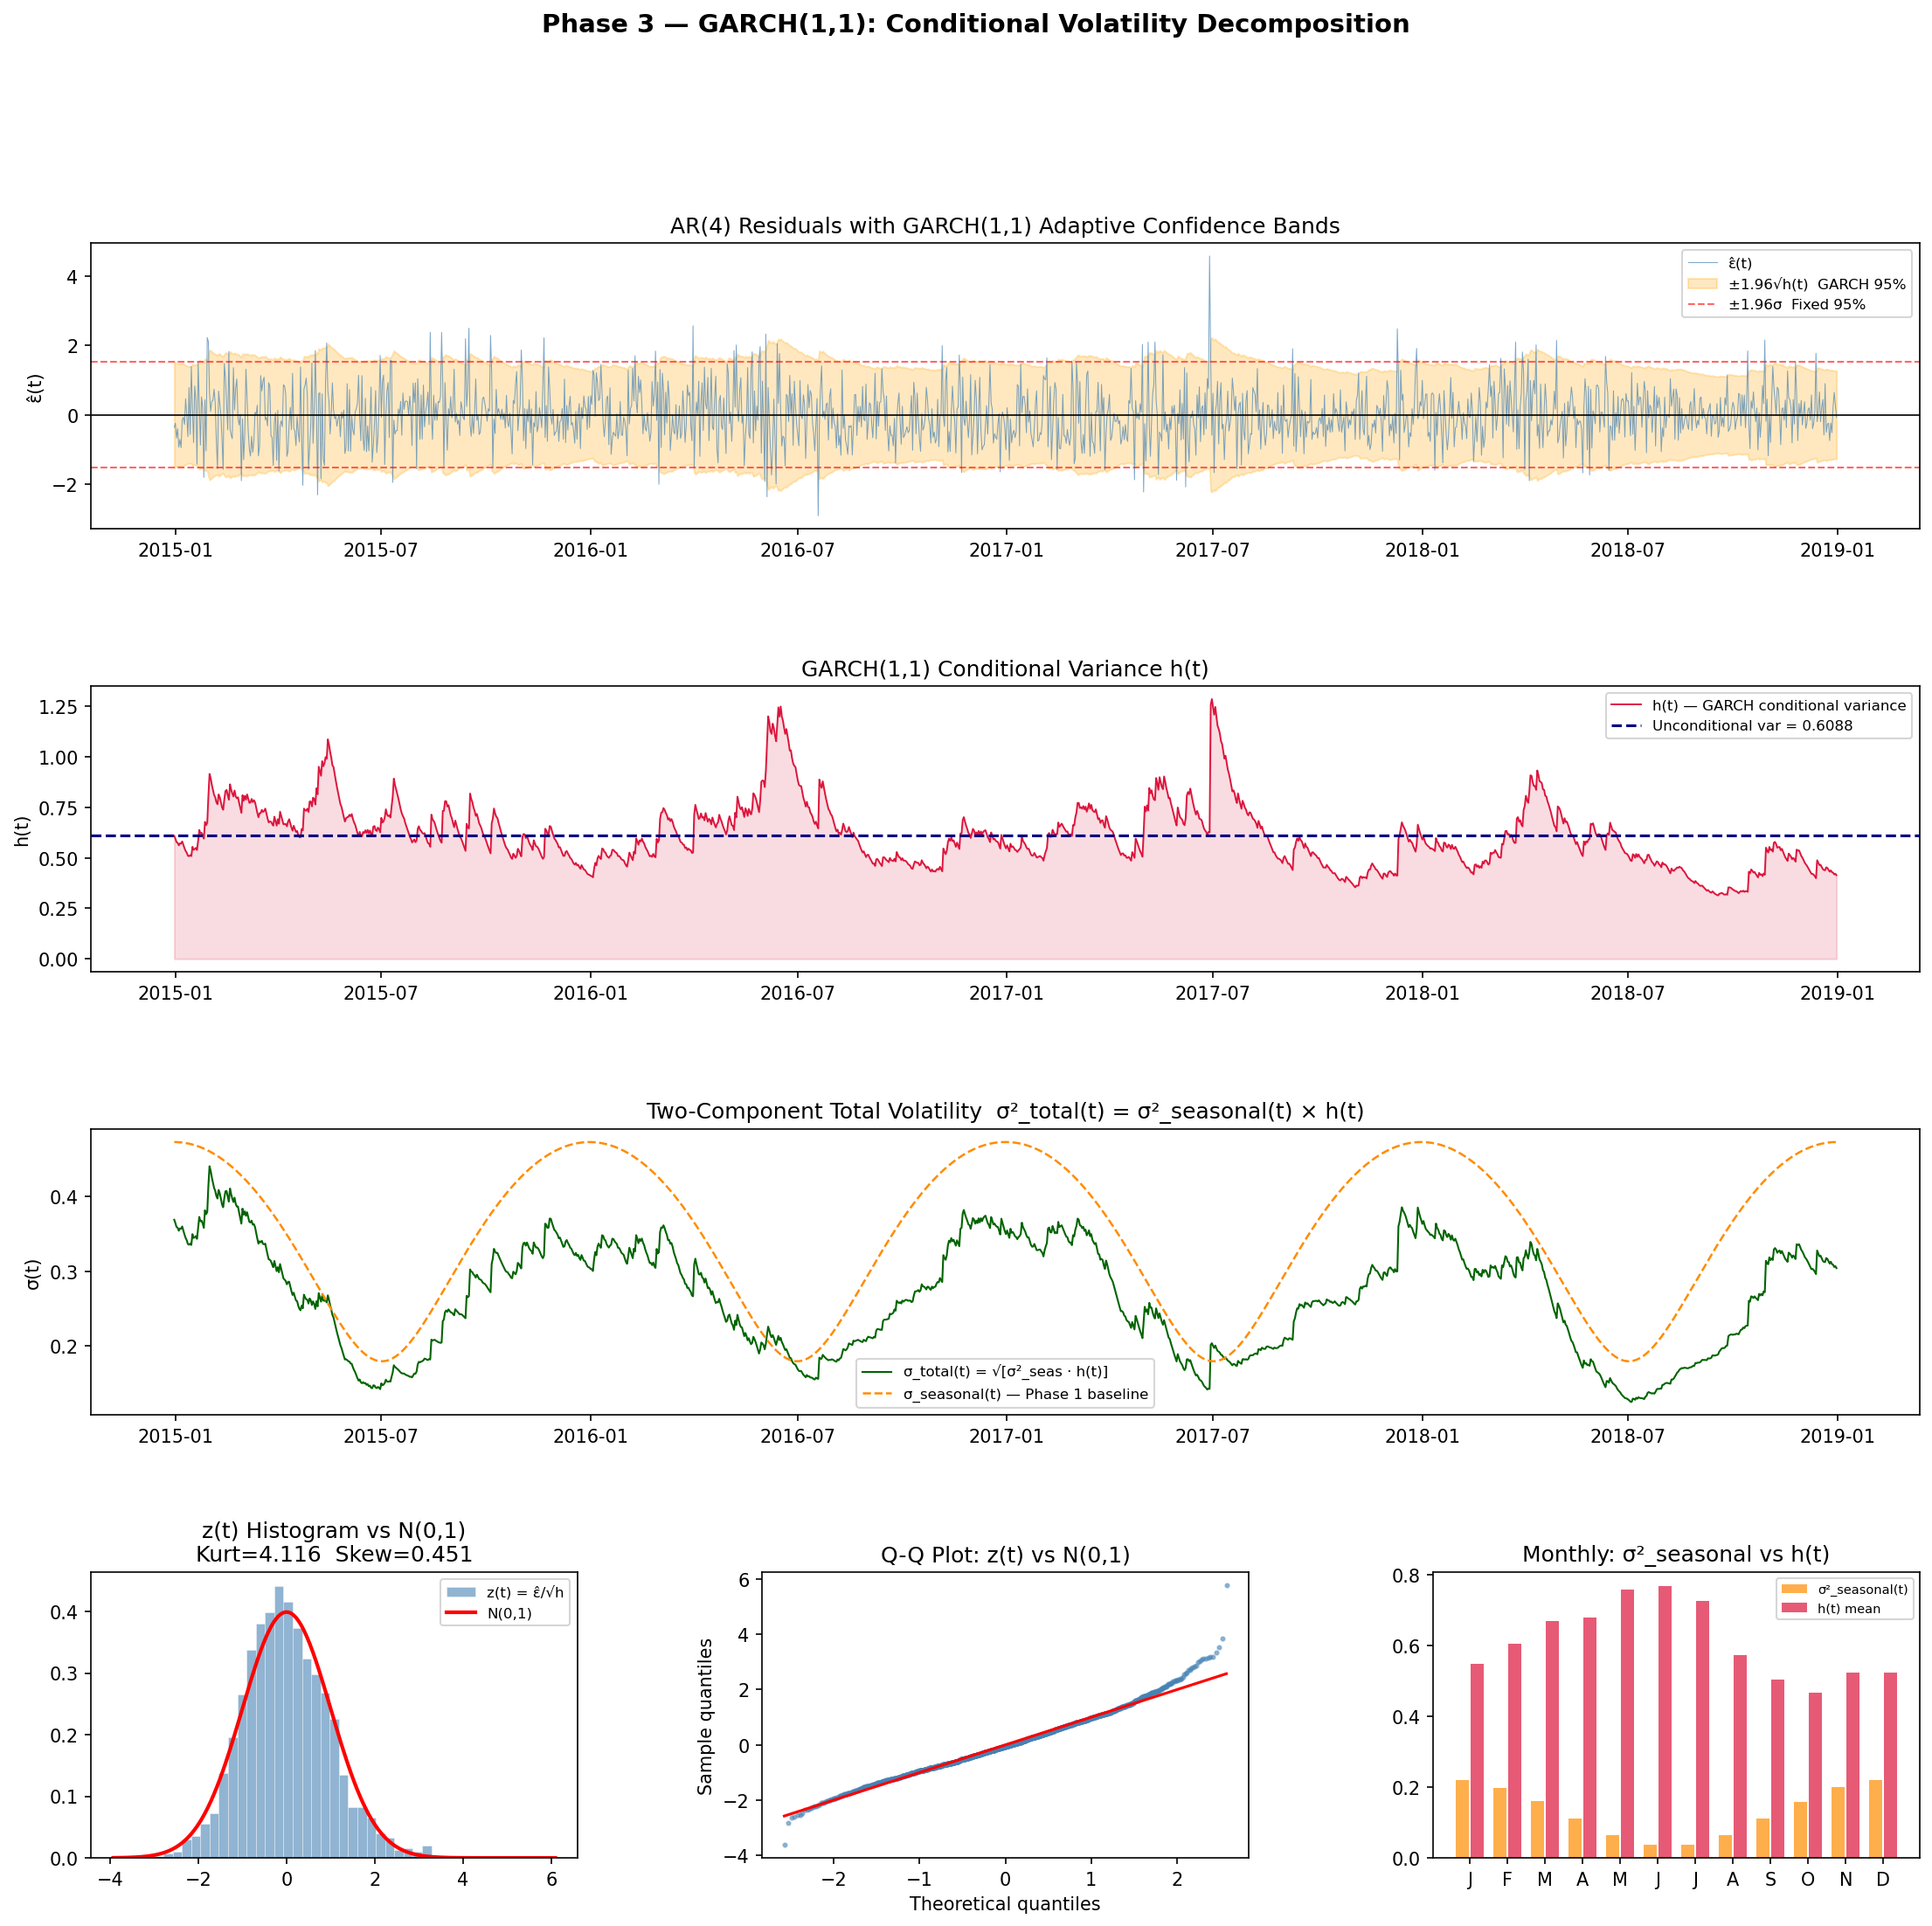
\includegraphics[width=\textwidth]{figures/phase3_garch_diagnostics.png}
\caption{Dataset A}
\end{subfigure}
\hfill
\begin{subfigure}{0.48\textwidth}
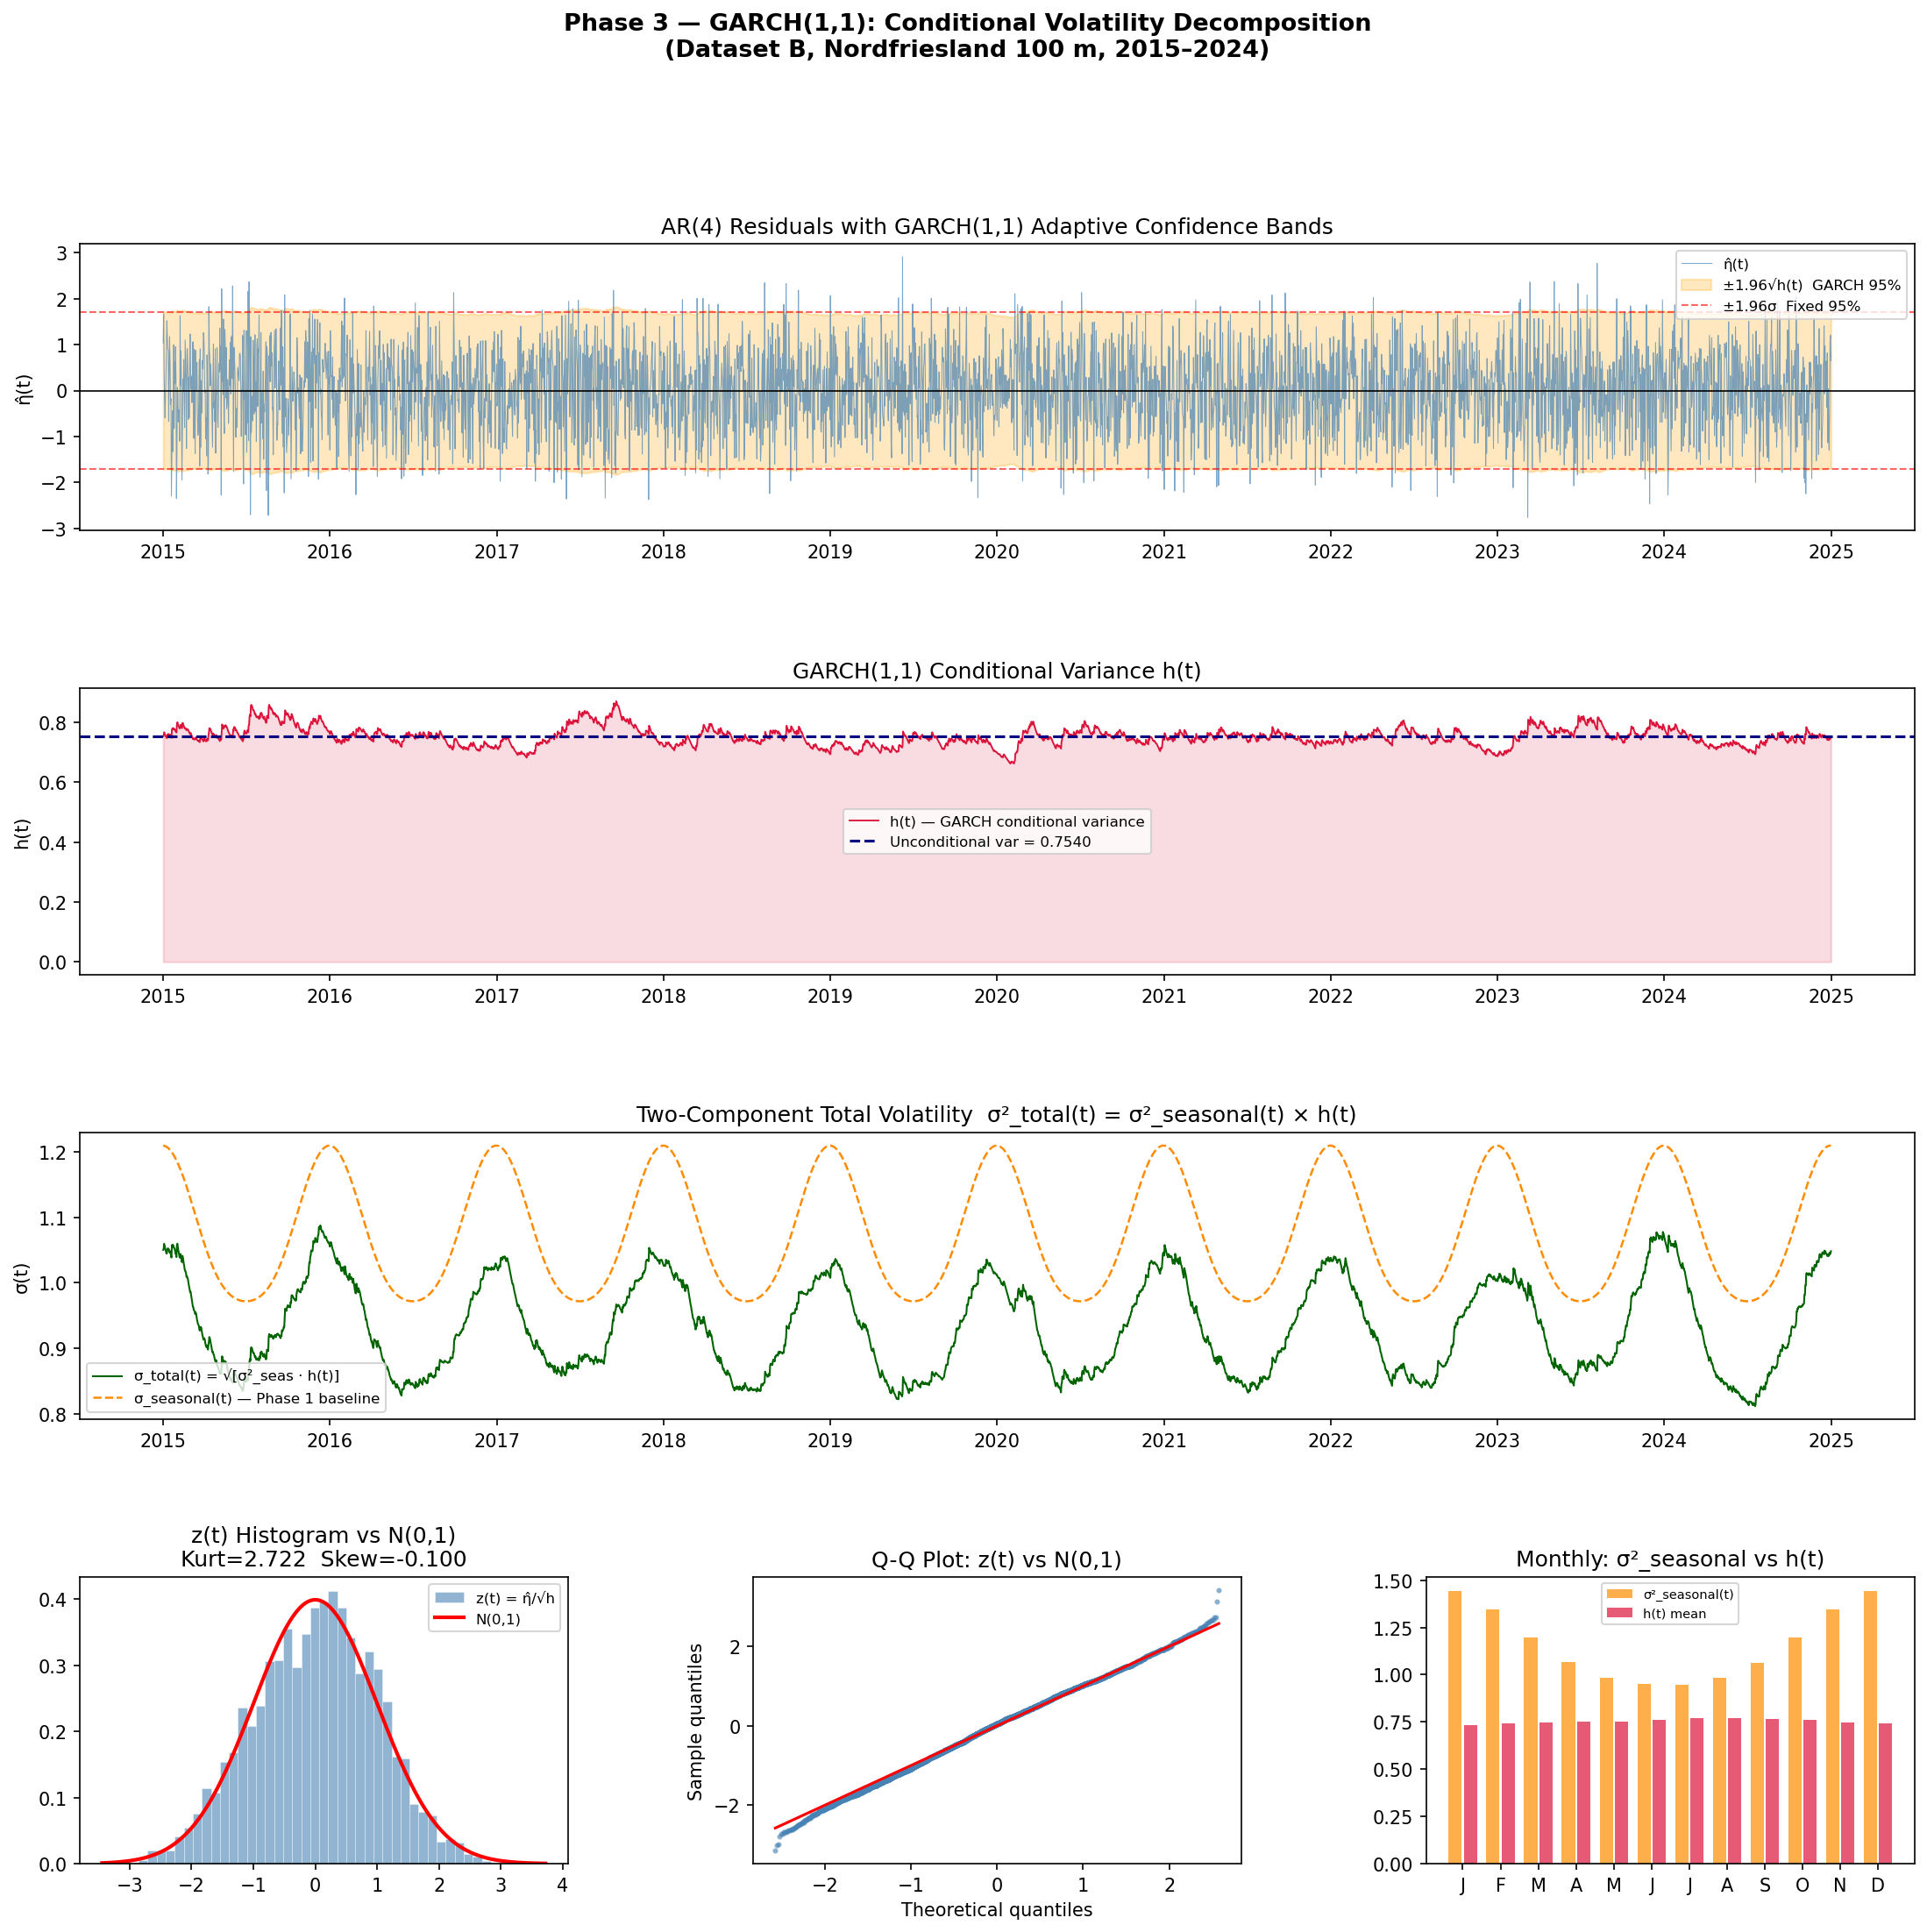
\includegraphics[width=\textwidth]{figures/phase3_B_garch_diagnostics.png}
\caption{Dataset B}
\end{subfigure}
\caption{GARCH(1,1) conditional-volatility decomposition, both datasets. Each panel is arranged in four rows. \textbf{Row 1:} the AR(4) residuals with GARCH-adaptive 95\% confidence bands ($\pm 1.96\sqrt{h(t)}$) plotted against fixed-width bands, visibly widening around high-volatility episodes. \textbf{Row 2:} the fitted conditional-variance path $h(t)$ against its unconditional long-run level. \textbf{Row 3:} the two-component total volatility $\sigma_{\text{total}}(t) = \sqrt{\sigma^2_{\text{seasonal}}(t)\, h(t)}$ against the Phase~1 seasonal baseline. \textbf{Row 4:} three panels -- a histogram of the standardised residuals $z(t)$ against the normal distribution; a quantile--quantile plot of $z(t)$ against the normal distribution; and a monthly bar-chart comparison of the seasonal-variance and GARCH components, illustrating the dataset-dependent degree to which the two effects offset each other, discussed in Section~\ref{sec:phase3-decomp}.}
\label{fig:phase3-garch}
\end{figure}

\subsection{Cross-Dataset Comparison}
\label{sec:phase3-compare}

Dataset B's own analysis draws an explicit comparison back to Dataset A, attributing its lower shock-sensitivity ($\alpha = 0.0059$ versus $0.0311$) and higher persistence-to-shock ratio ($\beta/\alpha = 165$ versus $31$) to more stable boundary-layer mixing at 100~m hub height relative to the 10~m surface layer, over a decade-long record rather than a four-year one. The physical mechanism behind that contrast is worth setting out explicitly, since it recurs at several points in this chapter. At 10~m, surface roughness, thermal convection, and diurnal heating cycles create highly turbulent, localised eddies that manifest as abrupt, short-lived volatility shocks. At 100~m, by contrast, measurements reside higher in the atmospheric boundary layer, closer to the geostrophic wind flow, where momentum is driven by large-scale pressure gradients rather than local surface friction; the result is a smoother conditional-variance regime, in which variance is carried forward from its own past level to a much greater degree than it is driven by fresh shocks. One phrase in that comparison is worth a precision note: Dataset B's total persistence $\alpha+\beta = 0.9821$ is in fact marginally \emph{lower} than Dataset A's $0.9835$, so the claim that Dataset B is ``more persistent'' rests on the $\beta$-to-$\alpha$ decomposition, not on $\alpha+\beta$ itself; this thesis reports the comparison on that more precise basis in Table~\ref{tab:garch} rather than repeating the aggregate persistence framing.

\section{Continuous-Time Embedding: CAR(4)}
\label{sec:phase4}

The AR(4) model of Section~\ref{sec:phase2} is fit on a daily grid, but a derivative contract must in general be priced at an arbitrary maturity that does not fall on that grid. This section embeds the discrete AR(4) model into a continuous-time CAR(4) state-space representation, following \citet{BenthSaltyteBenth2009} and the general Lévy-driven CARMA theory of \citet{BrockwellMarquardt2005}.

\subsection{Euler Discretisation and the Companion Matrix}
\label{sec:phase4-euler}

The mapping between the two representations is not an independent fit: it is the algebraic consequence of a single modelling choice, namely that the daily AR(4) recursion is itself what results from discretising the continuous-time CAR(4) stochastic differential equation, $\mathrm dX(t) = A\,X(t)\,\mathrm dt + e_4\,\sigma(t)\,\mathrm dB(t)$, by a first-order (Euler) finite-difference approximation taken at a one-day step size. Writing that finite-difference approximation out and matching it term by term against the discrete AR(4) equation yields four algebraic identities expressing the continuous-time coefficients $\{\alpha_1,\dots,\alpha_4\}$ directly in terms of the discrete $\{\beta_1,\dots,\beta_4\}$, given by \citet{BenthSaltyteBenth2009}: $\alpha_1 = 4-\beta_1$, $\alpha_2 = 3\alpha_1 - \beta_2 - 6$, $\alpha_3 = 4 + 2\alpha_2 - \beta_3 - 3\alpha_1$, $\alpha_4 = \alpha_3 - \beta_4 - \alpha_2 + \alpha_1 - 1$. Because the map is derived algebraically rather than fitted, it is invertible by construction, and for Dataset A this is verified directly: substituting the fitted $\alpha$ coefficients back through the inverse relations reproduces the original $\beta$ coefficients to machine precision ($\max|\beta_{\text{orig}} - \beta_{\text{reconstructed}}| = 7.77\times 10^{-16}$), confirming that no information is lost in either direction of the mapping. The resulting $\alpha$ coefficients populate the last row of the companion matrix
\begin{equation}
A = \begin{pmatrix} 0 & 1 & 0 & 0 \\ 0 & 0 & 1 & 0 \\ 0 & 0 & 0 & 1 \\ -\alpha_4 & -\alpha_3 & -\alpha_2 & -\alpha_1 \end{pmatrix},
\end{equation}
following the general companion-matrix construction of \citet{BrockwellMarquardt2005}. Table~\ref{tab:car4-alpha} reports the fitted coefficients for both datasets: Dataset B's coefficients are larger than Dataset A's at every lag, and the gap widens with lag order, from a 2.9\% difference at $\alpha_1$ to 5.3\% at $\alpha_2$, 9.4\% at $\alpha_3$, and 32.8\% at $\alpha_4$. The underlying analysis attributes the overall pattern to slower, more sluggish mean-reversion dynamics in the atmospheric boundary layer at 100~m relative to the 10~m surface layer, but does not separately account for the widening of the gap at higher lags. One physical hypothesis suggests itself, consistent with the boundary-layer contrast set out in Section~\ref{sec:phase3-compare}: higher-order lags in a continuous-time autoregression capture the persistence of older synoptic weather structures, and a gap that widens with lag order is what would be expected if the momentum of past pressure systems dissipates more slowly at 100~m than at the surface, where ground friction rapidly breaks down the ``memory'' of atmospheric conditions beyond a few days. This is offered as an interpretation of the fitted coefficients rather than as a separately tested result.

\begin{table}[htbp]
\centering
\caption{CAR(4) coefficients $\alpha_1,\dots,\alpha_4$, both datasets.}
\label{tab:car4-alpha}
\begin{tabular}{l r r}
\toprule
\textbf{Coefficient} & \textbf{Dataset A} & \textbf{Dataset B} \\
\midrule
$\alpha_1$ & $3.3701$ & $3.4676$ \\
$\alpha_2$ & $4.2546$ & $4.4789$ \\
$\alpha_3$ & $2.3063$ & $2.5228$ \\
$\alpha_4$ & $0.3908$ & $0.5188$ \\
\bottomrule
\end{tabular}
\end{table}

\subsection{Eigenvalues and Stationarity}
\label{sec:phase4-eigen}

Stationarity of the continuous-time system requires every eigenvalue of $A$ to have a strictly negative real part, the continuous-time analogue of the discrete unit-circle condition. Table~\ref{tab:car4-eigen} confirms this for both datasets. In both cases the eigenvalues comprise one complex-conjugate pair and two real values; the complex pair generates an oscillatory component in the impulse-response kernel (Section~\ref{sec:phase4-samuelson}) with periods that differ substantially across the two datasets: approximately 13.5 days for Dataset A ($2\pi/0.465$) and approximately 24.6 days for Dataset B ($2\pi/0.255$). Both are consistent with mid-latitude synoptic weather cycles, which span a 10--30-day range depending on the atmospheric-circulation pattern. The dominant (least negative) eigenvalue implies a mean-reversion half-life of 2.33 days for Dataset A, close to the 2.0-day half-life already found directly from the discrete AR(4) roots in Section~\ref{sec:phase2-coefs}. For Dataset B the dominant eigenvalue implies a half-life of 1.24 days, markedly faster than the roughly 40-day half-life of the GARCH volatility \emph{regime} found in Section~\ref{sec:phase3-estimates}. This distinction is worth stating explicitly, since the two numbers answer different questions: the CAR(4) eigenvalue governs how quickly the \emph{mean level} of a wind-speed anomaly reverts, while the GARCH persistence governs how quickly the \emph{variance regime} it occurred in reverts, and there is no reason to expect the two rates to coincide.

\begin{table}[htbp]
\centering
\caption{Eigenvalues of the CAR(4) companion matrix, both datasets.}
\label{tab:car4-eigen}
\begin{tabular}{l r r}
\toprule
& \textbf{Dataset A} & \textbf{Dataset B} \\
\midrule
Complex pair $\lambda_{c},\bar\lambda_{c}$ & $-0.9358 \pm 0.4653i$ & $-1.0730 \pm 0.2550i$ \\
Oscillatory period (days) & $13.5$ & $24.6$ \\
Real eigenvalue & $-1.2004$ & $-0.7614$ \\
Dominant (least negative) real eigenvalue & $-0.2980$ & $-0.5602$ \\
All $\mathrm{Re}(\lambda) < 0$? & \textbf{Yes} & \textbf{Yes} \\
Half-life, dominant mode (days) & $2.33$ & $1.24$ \\
\bottomrule
\end{tabular}
\end{table}

\subsection{Conditional Forecasts}
\label{sec:phase4-forecast}

Under the physical measure, the conditional mean and variance of the state vector at horizon $\tau$ are $\mathbb E[X(t_0+\tau)\mid\mathcal F_{t_0}] = e_1' \exp(A\tau) X(t_0)$ and $\mathrm{Var}[X_1(t_0+\tau)\mid\mathcal F_{t_0}] = \sigma^2_{\text{total}}(t_0)\int_0^\tau g(s)^2\,\mathrm ds$, where $g(s) = e_1'\exp(As)e_4$ is the impulse-response kernel and $\sigma^2_{\text{total}}(t_0)$ is the two-component variance of Section~\ref{sec:phase3-decomp}. Both datasets show a non-monotone conditional-mean path, a direct consequence of the oscillatory complex eigenpair: the forecast mean peaks a few days ahead of $t_0$ before decaying toward zero (Dataset A: peak at a 3-day horizon; Dataset B: peak at a 2-day horizon), rather than declining monotonically from the current state as a simple AR(1)/OU model would predict. Conditional variance saturates at its unconditional level within three to four weeks in both datasets (Dataset A: by a 21--30-day horizon; Dataset B: by a 14--21-day horizon), consistent with the half-lives of Table~\ref{tab:car4-eigen}. Table~\ref{tab:car4-forecast} reports the full term structure for both datasets, computed from the state vectors $X(t_0)_A = (0.1299, 0.5159, 0.4672, -0.3422)'$ and $X(t_0)_B = (1.3785, 1.4862, 0.4380, -1.3453)'$, the last four standardised observations of each sample.

The values in Table~\ref{tab:car4-forecast} reproduce the Phase~4 output exactly, but they cannot be read at face value as conditional forecasts of $\widetilde W(t)$, and the reasons are worth setting out rather than leaving for the reader to discover. Three of the table's implications conflict with results established elsewhere in this chapter. The conditional standard deviation at a one-day horizon is $0.009$ for Dataset A and $0.031$ for Dataset B, against one-step-ahead root mean squared errors of $0.6017$ and $0.8580$ for the same series in Table~\ref{tab:ar4-rmse}, a discrepancy of a factor of $67$ and $28$ respectively for what is nominally the same quantity. The conditional variance saturates at $0.247$ and $0.720$, against unconditional standard deviations of $0.967$ and $1.005$ reported for $\widetilde W(t)$ in Section~\ref{sec:phase1-wtilde}, so the embedding settles at roughly half the variance of the series it was fitted to. And the conditional mean for Dataset B rises from a current state of $X_1 = 1.3785$ to $2.845$ at one day and $3.610$ at two, with a one-day interval that would place tomorrow's standardised observation between roughly $2.8$ and $2.9$ standard deviations above the mean.

The oscillatory hump discussed above is a genuine property of the CAR($p \geq 2$) kernel and is not in question, but it does not account for excursions of this size alongside near-zero forecast uncertainty. A specific and testable explanation is available. The companion matrix of Equation~(4) defines its state components as successive derivatives, $X_{j+1} = \mathrm dX_j/\mathrm dt$, whereas the state vectors above are populated with successive \emph{lags} of $\widetilde W$. Propagating a lag-populated vector through $\exp(A\tau)$ built on the derivative convention treats the second component as a time derivative of the first, and the arithmetic is consistent with that reading: to first order, $[\exp(A)X]_1 \approx X_1 + X_2$, which for Dataset B gives $1.3785 + 1.4862 = 2.865$ against the tabulated $2.845$, the small remainder being the higher-order terms. The same mechanism would depress the apparent conditional variance, since the variance integral and the mean propagator would then be parameterised inconsistently. Resolving this requires re-running the Phase~4 conditional-forecast step under a consistent state-space convention, which is outside the scope of a chapter that treats the phase outputs as frozen; the table is therefore retained as the recorded output, and its horizon profile should be read as indicative of the shape of the CAR(4) response rather than as a calibrated predictive interval. The qualitative conclusions this chapter draws from it, the non-monotone mean path and the saturation of variance within three to four weeks, do not depend on the absolute scale of either column.

\begin{table}[htbp]
\centering
\small
\caption{CAR(4) conditional-mean forecast term structure, both datasets.}
\label{tab:car4-forecast}
\begin{tabular}{l r r r r}
\toprule
& \multicolumn{2}{c}{\textbf{Dataset A}} & \multicolumn{2}{c}{\textbf{Dataset B}} \\
\textbf{Horizon (days)} & \textbf{Mean} & \textbf{Std.\ dev.} & \textbf{Mean} & \textbf{Std.\ dev.} \\
\midrule
1 & $0.779$ & $0.009$ & $2.845$ & $0.031$ \\
2 & $1.303$ & $0.052$ & $3.610$ & $0.172$ \\
3 & $1.460$ & $0.110$ & $3.497$ & $0.358$ \\
5 & $1.113$ & $0.197$ & $2.146$ & $0.614$ \\
7 & $0.658$ & $0.232$ & $0.983$ & $0.699$ \\
10 & $0.270$ & $0.245$ & $0.237$ & $0.719$ \\
14 & $0.082$ & $0.247$ & $0.029$ & $0.720$ \\
21 & $0.010$ & $0.247$ & $0.001$ & $0.720$ \\
30 & $0.001$ & $0.247$ & $\approx 0$ & $0.720$ \\
\bottomrule
\end{tabular}
\end{table}

\subsection{Normal-Inverse-Gaussian Tails}
\label{sec:phase4-nig}

Section~\ref{sec:phase3-diag} found that GARCH-standardised residuals depart from normality in both datasets, in opposite directions: leptokurtic for Dataset A, platykurtic for Dataset B. This motivates fitting a Normal-Inverse-Gaussian (NIG) distribution to the standardised residuals as a heavy-tailed alternative to the Gaussian innovation assumed elsewhere in this chapter, following \citet{BarndorffNielsenShephard2001}. Table~\ref{tab:nig} reports the fit. For Dataset A the NIG tail-heaviness parameter $\hat\alpha = 4.374$ is small (heavy tails) and the fit is a modest but genuine improvement over the Gaussian (Kolmogorov--Smirnov $p = 0.120$ versus $0.079$), though it still falls short of the full empirical kurtosis, an outstanding gap attributed largely to the single 28~June~2017 extreme observation identified in Section~\ref{sec:phase3-diag}. This implies that the heavy-tailed NIG extension for Dataset A is largely an artefact of a single meteorological anomaly: were that event excluded, the residual distribution would be expected to collapse back toward a Gaussian profile, which further supports retaining the Gaussian CAR(4) framework as the primary pricing track. No such re-estimation is performed here, consistent with this chapter's treatment of the phase results as frozen, so this remains an inference from the fitted diagnostics rather than a demonstrated result. For Dataset B the fitted $\hat\alpha \approx 2{,}650$ is enormous, reflecting a body so close to Gaussian that the NIG fit offers no material improvement over the normal (KS $p = 0.0275$ versus $0.0269$ for the Gaussian). Both fits give a skewness parameter $\hat\beta$ close to zero (Dataset A: $0.0067$, freely estimated rather than constrained; Dataset B: $-0.0021$), consistent with approximately symmetric innovations in both datasets. Given this asymmetry in how much the NIG assumption actually buys, the Gaussian CAR(4) specification is retained as the primary pricing track for Chapter~3 in both datasets, consistent with \citet{BenthSaltyteBenth2009}; the NIG fit is carried forward as a documented robustness extension, using the closed-form NIG moment-generating function of \citet{BrockwellMarquardt2005}, rather than as the operative model.

\begin{table}[htbp]
\centering
\caption{Normal-Inverse-Gaussian fit to standardised GARCH residuals, both datasets.}
\label{tab:nig}
\begin{tabular}{l r r}
\toprule
\textbf{Parameter} & \textbf{Dataset A} & \textbf{Dataset B} \\
\midrule
$\hat\alpha$ (tail heaviness) & $4.374$ & $2{,}649.57$ \\
$\hat\beta$ (asymmetry) & $0.0067$ & $-0.0021$ \\
$\hat\delta$ (scale) & $2.087$ & $51.516$ \\
$\hat\mu$ (location) & $0.000$ & $0.000$ \\
Empirical excess kurtosis of $z(t)$ & $+1.116$ & $-0.278$ \\
KS $p$ (NIG / Gaussian) & $0.120$ / $0.079$ & $0.0275$ / $0.0269$ \\
\bottomrule
\end{tabular}
\end{table}

\begin{figure}[htbp]
\centering
\begin{subfigure}{0.48\textwidth}
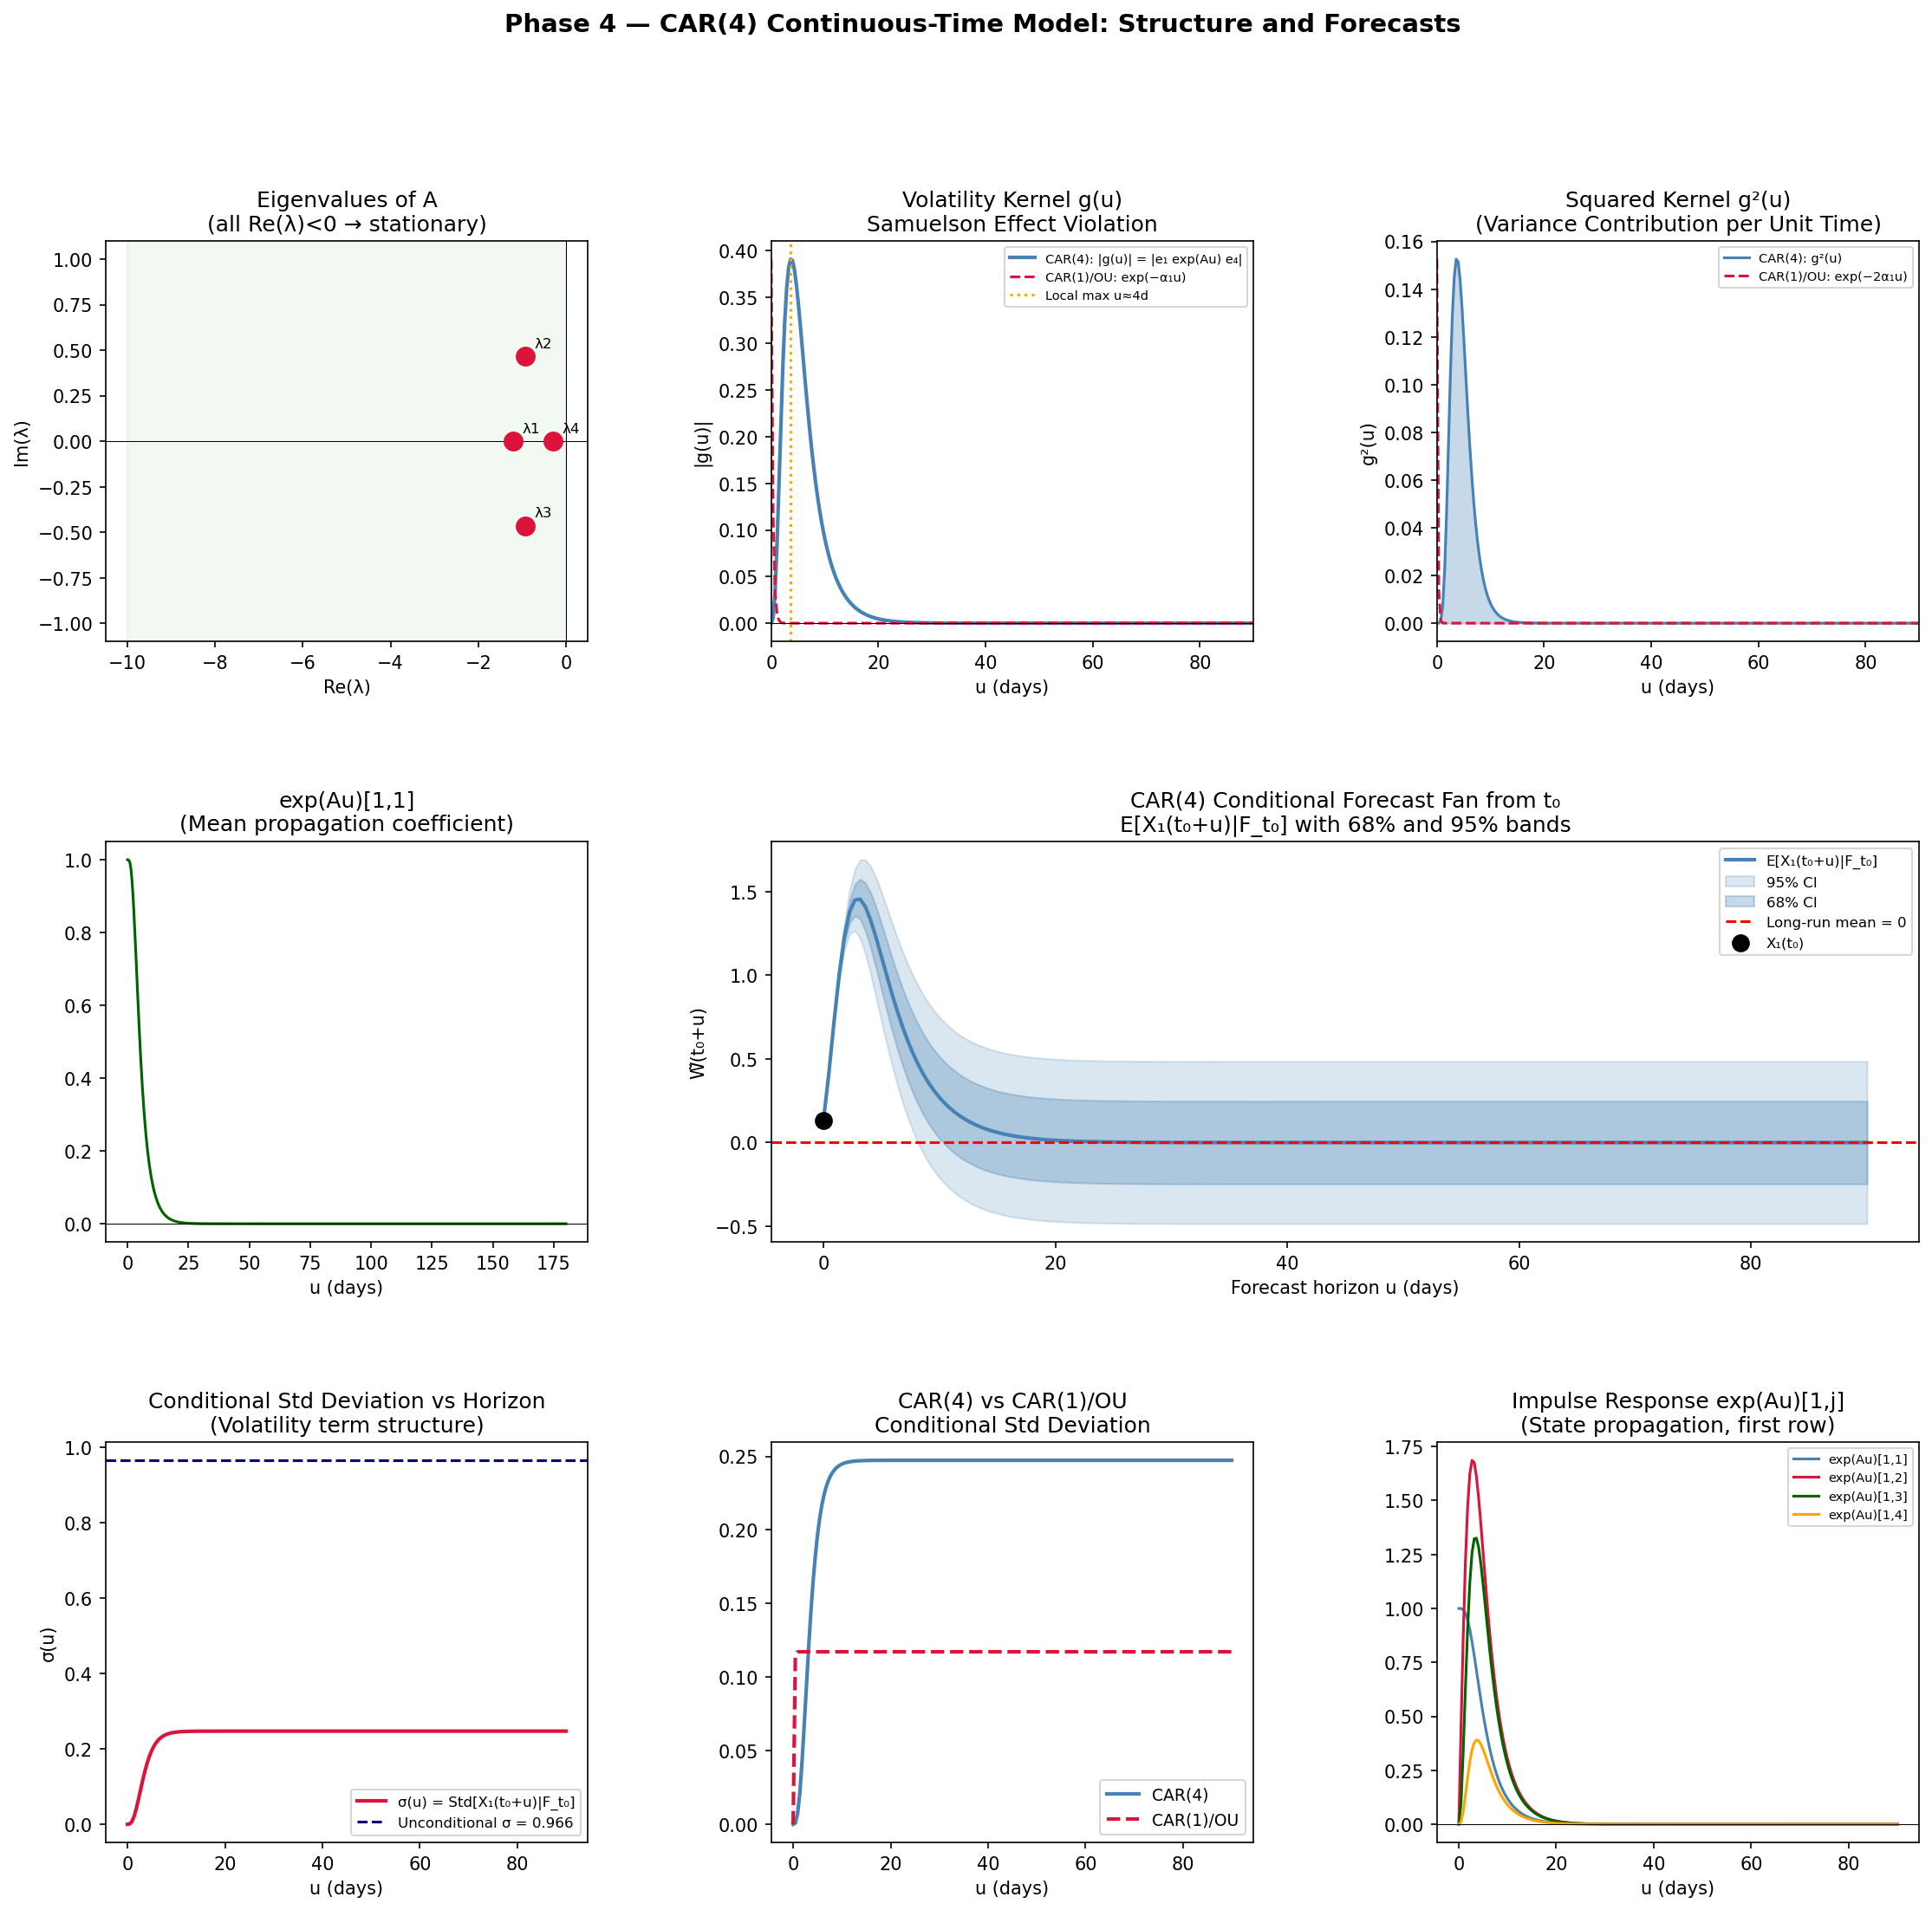
\includegraphics[width=\textwidth]{figures/phase4_car4_analysis.png}
\caption{Dataset A}
\end{subfigure}
\hfill
\begin{subfigure}{0.48\textwidth}
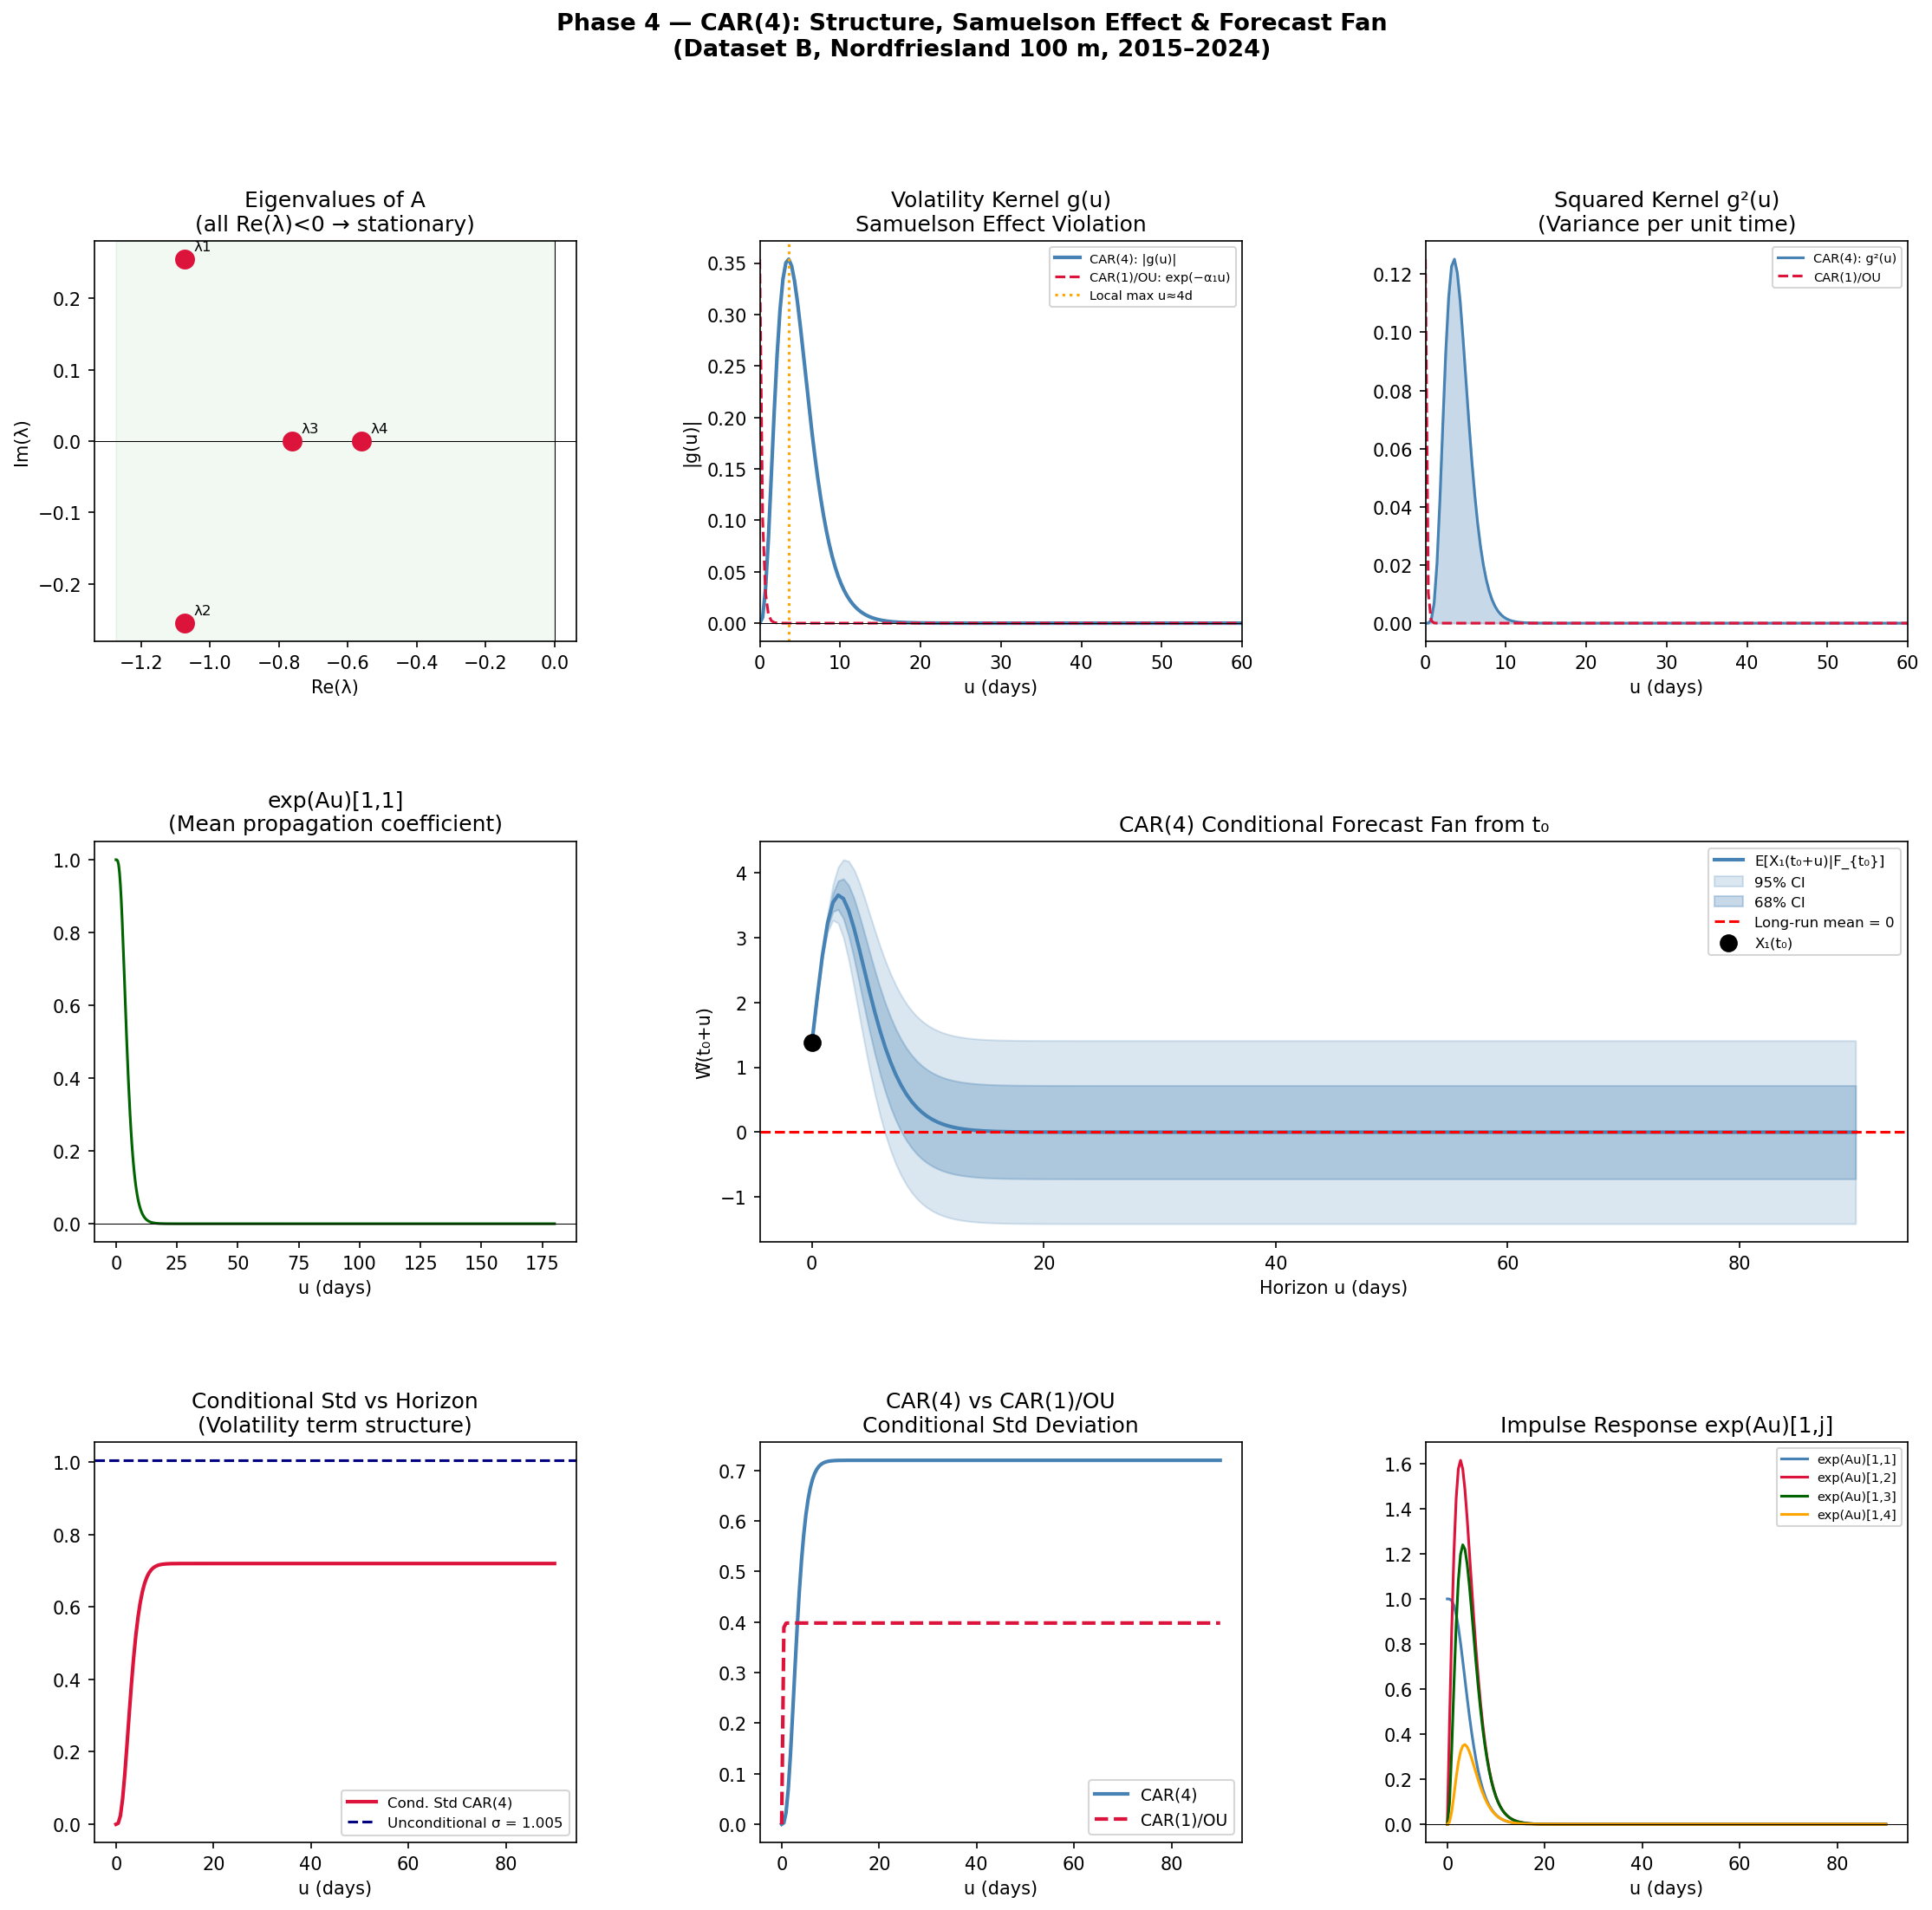
\includegraphics[width=\textwidth]{figures/phase4_B_car4_analysis.png}
\caption{Dataset B}
\end{subfigure}
\caption{CAR(4) structure and conditional forecasts, both datasets. Each panel is arranged in three rows. \textbf{Row 1:} three panels -- the eigenvalues of the companion matrix $A$ plotted in the complex plane (all in the open left half-plane, confirming stationarity); the impulse-response kernel $g(u) = e_1'\exp(Au)e_4$ against the monotone CAR(1)/Ornstein--Uhlenbeck baseline, showing the local maximum near a 3.6-day horizon that drives the Samuelson-effect violation of Section~\ref{sec:phase4-samuelson}; and the squared kernel $g(u)^2$. \textbf{Row 2:} two panels -- the $[\exp(Au)]_{11}$ mean-propagation curve, and the conditional-forecast fan (mean, with 68\% and 95\% bands) built forward from the current state $X(t_0)$. \textbf{Row 3:} three panels -- the conditional standard deviation against horizon, saturating at its unconditional level; a comparison of the CAR(4) and CAR(1) variance term structures; and the full first-row impulse-response matrix $[\exp(Au)]_{1j}$ across all four state components.}
\label{fig:phase4-car4}
\end{figure}

\subsection{Seasonal Variance Carried Forward}
\label{sec:phase4-c0}

The Fourier seasonal-variance constant $C_0$ used throughout this chapter and in Chapter~3 is a Phase~1 result (Section~\ref{sec:phase1-seasonal}), not re-estimated at this stage: Dataset B's Phase~4 output carries $C_0, C_1, C_2$ forward explicitly alongside the CAR(4) parameters, reproducing $C_0 = 1.163$ to the precision of the frozen anchor, while Dataset A's corresponding output records only the point value $\sigma^2_{\text{seasonal}}(t_0) = 0.2239$ and does not separately re-list $C_0$. Both are consistent with $C_0 = 0.13138$; the value is simply carried through from Section~\ref{sec:phase1-seasonal} rather than recomputed, and this thesis does not treat its absence from Dataset A's Phase~4 output as a gap, since CAR(4) has no reason to refit a quantity that Phase~1 has already fixed.

\subsection{The Samuelson Effect}
\label{sec:phase4-samuelson}

A single-factor Ornstein--Uhlenbeck model ($p=1$, the Schwartz~\citeyearpar{Schwartz1997} special case) has an impulse-response kernel $g(u) = e^{-\alpha_1 u}$ that decays monotonically, and futures volatility built on that kernel therefore rises monotonically as maturity approaches: the classical Samuelson effect. The complex eigenvalue pair found in both datasets' CAR(4) systems (Table~\ref{tab:car4-eigen}) breaks this monotonicity: the kernel $g(u)$ attains a local maximum at a horizon of roughly 3.6 days in both datasets before declining, so that shocks occurring three to four days before contract settlement have \emph{more}, not less, impact on terminal volatility than shocks occurring closer to settlement. \citet{BenthSaltyteBenth2009} derive this violation analytically for Nordix wind futures; the same qualitative pattern is confirmed numerically here for both Dataset A and Dataset B, despite their different fitted coefficients, which suggests the effect is a structural property of the CAR($p\geq2$) kernel rather than an artefact of either specific site.

\section{Stochastic-Volatility Framework}
\label{sec:phase5}

The GARCH(1,1) filter of Section~\ref{sec:phase3} is a valid discrete-time description of conditional heteroskedasticity, but it cannot serve directly as the volatility driver of a continuous-time pricing model. This section embeds it into a Heston-type \citep{Heston1993} stochastic-volatility system, following the same construction for both datasets; the treatment is theoretical throughout, for reasons explained in Section~\ref{sec:phase5-mle}, and no parameters are estimated beyond the GARCH proxy mapping.

\subsection{Motivation}
\label{sec:phase5-motivation}

Two obstacles prevent the GARCH recursion $h(t) = \omega + \alpha\hat\eta^2(t-1) + \beta h(t-1)$ from being used directly in a continuous-time pricing framework. First, the Feynman--Kac theorem links a derivative's price to an expectation under a diffusion's dynamics precisely because that diffusion possesses a well-defined infinitesimal generator, the operator that encodes its instantaneous drift and diffusion; a GARCH path, updated once per day by a deterministic rule with no diffusion term of its own, has zero quadratic variation between updates and is therefore not a semimartingale, so no such generator exists and the Feynman--Kac correspondence between a pricing PDE and an expectation simply has nothing to act on. Second, a formal change of measure from the physical measure $P$ to a pricing measure $Q$, in the sense of Girsanov's theorem, works by shifting the drift of a Brownian motion that drives the process being repriced; the GARCH filter has no such driving Brownian motion to shift; it is a deterministic function of past innovations, so there is no drift for a change of measure to act on. The remedy, following \citet{Heston1993} and, for the specific application to wind speed, the CAR$(p)$ framework of \citet{BenthSaltyteBenth2009} and the Lévy-driven continuous-time machinery of \citet{BrockwellMarquardt2005}, is to embed the GARCH filter $h(t)$ into a Cox--Ingersoll--Ross (CIR) diffusion for a continuous-time variance process $V(t)$, which by construction is a semimartingale driven by its own Brownian motion, with the GARCH parameters entering as moment-matching proxies for the CIR parameters.

\subsection{Two-SDE System Under $P$}
\label{sec:phase5-sde}

For analytical tractability, the wind-speed dynamics are first written in a simplified CAR(1) form, with the full CAR(4) state-vector generalisation given afterward:
\begin{align}
\mathrm d\widetilde W(t) &= -\alpha_1 \widetilde W(t)\, \mathrm dt + \sqrt{V(t)}\, \mathrm dB_1(t), \\
\mathrm dV(t) &= \kappa_V(\bar v - V(t))\, \mathrm dt + \xi \sqrt{V(t)}\, \mathrm dB_2(t), \qquad \langle \mathrm dB_1, \mathrm dB_2\rangle_t = \rho\, \mathrm dt,
\end{align}
where $\alpha_1$ is the dominant CAR(4) mean-reversion parameter from Section~\ref{sec:phase4} ($\alpha_1 = 3.3701$ for Dataset A, $\alpha_1 = 3.4676$ for Dataset B), $\kappa_V$ is the mean-reversion speed of volatility, $\bar v$ the long-run variance, and $\xi$ the volatility-of-volatility coefficient. The full state-vector generalisation replaces the scalar drift with $\mathrm dX(t) = A\, X(t)\, \mathrm dt + e_4 \sqrt{V(t)}\, \mathrm dB_1(t)$, where $A$ is the $4\times4$ companion matrix of Section~\ref{sec:phase4} and $e_4 = (0,0,0,1)'$ injects the diffusion term through the newest lag, consistent with the state-space structure of the discretised CAR(4) model.

\subsection{Feller Condition}
\label{sec:phase5-feller}

The CIR process for $V(t)$ remains strictly positive almost surely if and only if the Feller condition $2\kappa_V \bar v > \xi^2$ holds; if it is violated, the diffusion term can dominate the mean-reverting drift near the origin and $V(t)$ can reach and remain at zero. The GARCH parameters of Section~\ref{sec:phase3-estimates} are mapped to CIR proxies by moment matching, $\kappa_V \approx 1-(\alpha+\beta)$, $\bar v \approx \omega/(1-\alpha-\beta)$, and $\xi^2 \approx \mathrm{Var}[h(t)]$, exactly as specified for the numerical Feller check permitted within the scope of this theoretical chapter. For Dataset B, this gives $\kappa_V = 0.0179$, $\bar v = 0.7522$, $\xi^2 = 0.000959$, so that $2\kappa_V\bar v = 0.0270$ comfortably exceeds $\xi^2$: the Feller condition holds with a margin of $28.1\times$.

For Dataset A, the same moment-matching procedure, applied with the same estimator, gives $\kappa_V = 0.0165$ and $\bar v = 0.608$, but $\xi^2 = \mathrm{Var}[h(t)] = 0.0253$, the full-sample variance of the Dataset A $h(t)$ series computed exactly as it was for Dataset B. Substituting into the condition gives $2\kappa_V\bar v = 0.0201$, which is \emph{smaller} than $\xi^2$: the Feller condition is violated, with a margin of $0.8\times$. Unlike Dataset B, the theoretical CIR embedding of this chapter is therefore not well posed for the proxy dataset on this specific numerical check.

This reverses the verdict recorded in the project specification, which lists a Feller margin of $27.9\times$ (holding) for Dataset A alongside $\xi^2 \approx 0.000048$; the reversal is stated here rather than reconciled silently. Three observations bear on it. First, the two specification figures are not consistent with each other: given $2\kappa_V\bar v = 0.0201$, a $\xi^2$ of $0.000048$ implies a margin of roughly $418\times$, not $27.9\times$. Second, neither figure is reproducible from the Phase~5 Dataset A source analysis, whose own executed output records $\xi^2 = 0.025264$ and returns the verdict as violated at $0.8\times$. Third, a $\xi^2$ of $0.000048$ would imply a standard deviation of $h(t)$ of approximately $0.007$, which cannot be reconciled with the monthly means of $h(t)$ reported in Section~\ref{sec:phase3-decomp}, which themselves range from $0.465$ to $0.768$. Rolling-window alternatives to the full-sample variance were examined as a possible explanation and do not recover the specification value either: a 30-day rolling standard deviation of $h(t)$ yields margins in the region of four to five times, still a violation. The specification figure is therefore treated here as an erratum rather than as a competing estimator, and the full-sample result is reported in the main text above.

The practical implication is the one developed at greater length in Section~\ref{sec:phase5-mle}. Of the four CIR proxies, $\xi$ is by some margin the least well identified at daily frequency, and a well-posedness verdict that inverts according to which estimator of $\mathrm{Var}[h(t)]$ is adopted is itself evidence of how weakly the volatility-of-volatility parameter is pinned down by daily data. The Feller check is reported here because the specification calls for it, but it should be read as a diagnostic of the proxy mapping rather than as a structural property of the underlying process.

This violation is not a modelling failure so much as a direct symptom of the proxy dataset's site characteristics. Dataset A (10~m) is heavily influenced by boundary-layer friction and local diurnal anomalies, producing the leptokurtic residual distribution and the single extreme shock already identified in Section~\ref{sec:phase3-diag} (the $5.79\sigma$ event of 28~June~2017). In a GARCH filter with the comparatively high shock sensitivity estimated for Dataset A ($\alpha = 0.0311$, against $0.0059$ for Dataset B), an outlier of that size produces a sharp, transient spike in $h(t)$, exactly the kind of feature that inflates a sample-variance-based $\xi^2$ proxy computed directly from the $h(t)$ path. Dataset B, measured at 100~m in the free atmosphere and free of any comparable shock, produces a markedly smoother $h(t)$ path and comfortably clears the condition instead. The asymmetry is informative in its own right, distinct from and additional to the pricing-error evidence of Chapter~3: the theoretical stochastic-volatility embedding developed in this chapter is well posed for the reference dataset and is not well posed, on this specific check, for the geographic proxy.

\subsection{Remark on the Change of Measure}
\label{sec:phase5-measure}

A formal change of measure from $P$ to a pricing measure $Q$ would introduce market-price-of-risk parameters $\theta_1, \theta_2$ shifting the drifts of $B_1$ and $B_2$, with $\kappa_V^Q = \kappa_V + \theta_2\xi$ under $Q$. This thesis adopts $\theta_1 = \theta_2 = 0$ throughout as a benchmark assumption, in the absence of EEX option-implied data, for two reasons that hold identically for both datasets. First, SMARD daily wind generation is a measured physical quantity, not a traded financial asset; the replication argument that pins down a unique risk-neutral measure for a traded derivative does not apply here, since no self-financing hedging portfolio in the underlying exists. Second, the only actively traded wind derivatives, the Nordix futures, reference Norwegian rather than German wind, and the geographic mismatch (Bologna or Nordfriesland versus Norway) prevents any clean calibration of $\theta$ from that market even in principle. Under $\theta = 0$, $P = Q$, and Track~A (empirical realised variance) and Track~B (model-implied variance) are defined on a common measure; the variance-swap fair strike of Chapter~3 reduces to the closed-form expression $K_{\text{var}}^B = h(t_0) \times C_0$, derived in Section~\ref{sec:phase3-decomp} from the Fourier decomposition under the piecewise-constant convention of \citet{Tol1997}, and no Girsanov computation is required anywhere in this thesis. This benchmark is adopted as a tractable simplification given the absence of option-implied data for this specific underlying, not as a claim that the market price of risk for wind-linked instruments is in fact zero.

\subsection{Characteristic Function and Round-Trip Consistency}
\label{sec:phase5-charfn}

Under the two-SDE system, the log-characteristic function of $\widetilde W(T)$ conditional on $\mathcal F_t$ takes the Heston \citeyearpar{Heston1993} form $\log\phi(u;t,T) = iu\,\mathbb E[\widetilde W(T)\mid\mathcal F_t] + C(\tau;u)\bar v + D(\tau;u) V(t)$, $\tau = T-t$, where $C$ and $D$ satisfy a coupled Riccati system, an ordinary differential equation containing a quadratic term in $D$, arising because the volatility process enters its own diffusion coefficient through $\sqrt{V(t)}$. This is what makes the system harder to solve than the linear CAR(4) dynamics of Section~\ref{sec:phase4}, whose companion-matrix ODE is solved exactly by the matrix exponential $\exp(A\tau)$: a Riccati equation has no such generic closed-form solution and instead requires the specific change-of-variables technique that Heston \citeyearpar{Heston1993} derives for this model, exploiting its particular algebraic structure rather than a general linear-systems result. Heston's closed-form solution defines $C$ and $D$ via complex square roots and logarithms, a substantially more delicate object to evaluate numerically than the CAR(4) matrix exponential used elsewhere in this chapter, since a careless implementation can pick the wrong branch of the complex logarithm and return a discontinuous, incorrect path as $\tau$ varies.

Under the $\theta=0$ benchmark, the first moment collapses to $\mathbb E[\widetilde W(T)\mid\mathcal F_t] = e_1' \exp(A\tau)X(t)$, exactly the CAR(4) conditional-mean forecast of Section~\ref{sec:phase4}. It is worth being precise about what this identity does and does not test: because $\theta = 0$ removes $C$ and $D$ from the first moment entirely, leaving only the linear companion-matrix propagator, the round-trip check that follows verifies the drift structure common to both representations, not the numerical handling of $C$ and $D$ themselves, which enter only the variance and higher moments of the characteristic function and are not separately checked here. This identity is verified numerically for both datasets by comparing the characteristic function's first moment against the Phase~4 conditional-forecast table at eleven horizons from 1 to 90 days: the maximum absolute discrepancy is $4.44\times 10^{-16}$ in both datasets, machine precision, confirming that the stochastic-volatility embedding's drift term is numerically consistent with the discrete CAR(4) forecasts it is built to extend, independently of the Feller-condition question raised above.

\subsection{Variance Term Structure}
\label{sec:phase5-termstructure}

The CAR(4) kernel $g(s) = e_1' \exp(As)e_4$ satisfies $g(0) = 0$: new information enters only through the most recent of the four lagged state components, and must propagate forward before it reaches the first. As a result, the variance term structure obtained under the piecewise-constant-$h$ convention of \citet{Tol1997}, $\mathrm{Var}^Q[\widetilde W(T)\mid\mathcal F_t] = h(t_0)\,\sigma^2_{\text{seasonal}}(t_0) \int_0^\tau g(s)^2\,\mathrm ds$, starts at zero and ramps up slowly. A simplified Heston/CIR term structure built on the CAR(1) reduction of Section~\ref{sec:phase5-sde} instead uses a kernel $g(s) = e^{-\alpha_1 s}$ that starts at one, producing an immediate jump in short-horizon variance. For Dataset B, the two term structures differ by a factor of roughly four at a one-day horizon (Tol/CAR(4): $0.00247$; Heston/CAR(1): $0.00985$) and converge only beyond a roughly two-week horizon, after which the ratio of the CAR(4) to the CAR(1) term structure settles in the $0.57$--$0.93$ range through 90 days. The two ratios quoted here are stated in the same direction, CAR(4) relative to CAR(1), the first being approximately $0.25$. The same qualitative pattern holds for Dataset A. This divergence is not a modelling inconsistency between the two approximations; it reflects a genuine structural feature of the CAR(4) state-space representation, and it is a first-order consideration for any option or short-dated instrument priced off the CAR(4) kernel rather than the simplified CAR(1) proxy.

\begin{figure}[htbp]
\centering
\begin{subfigure}{0.48\textwidth}
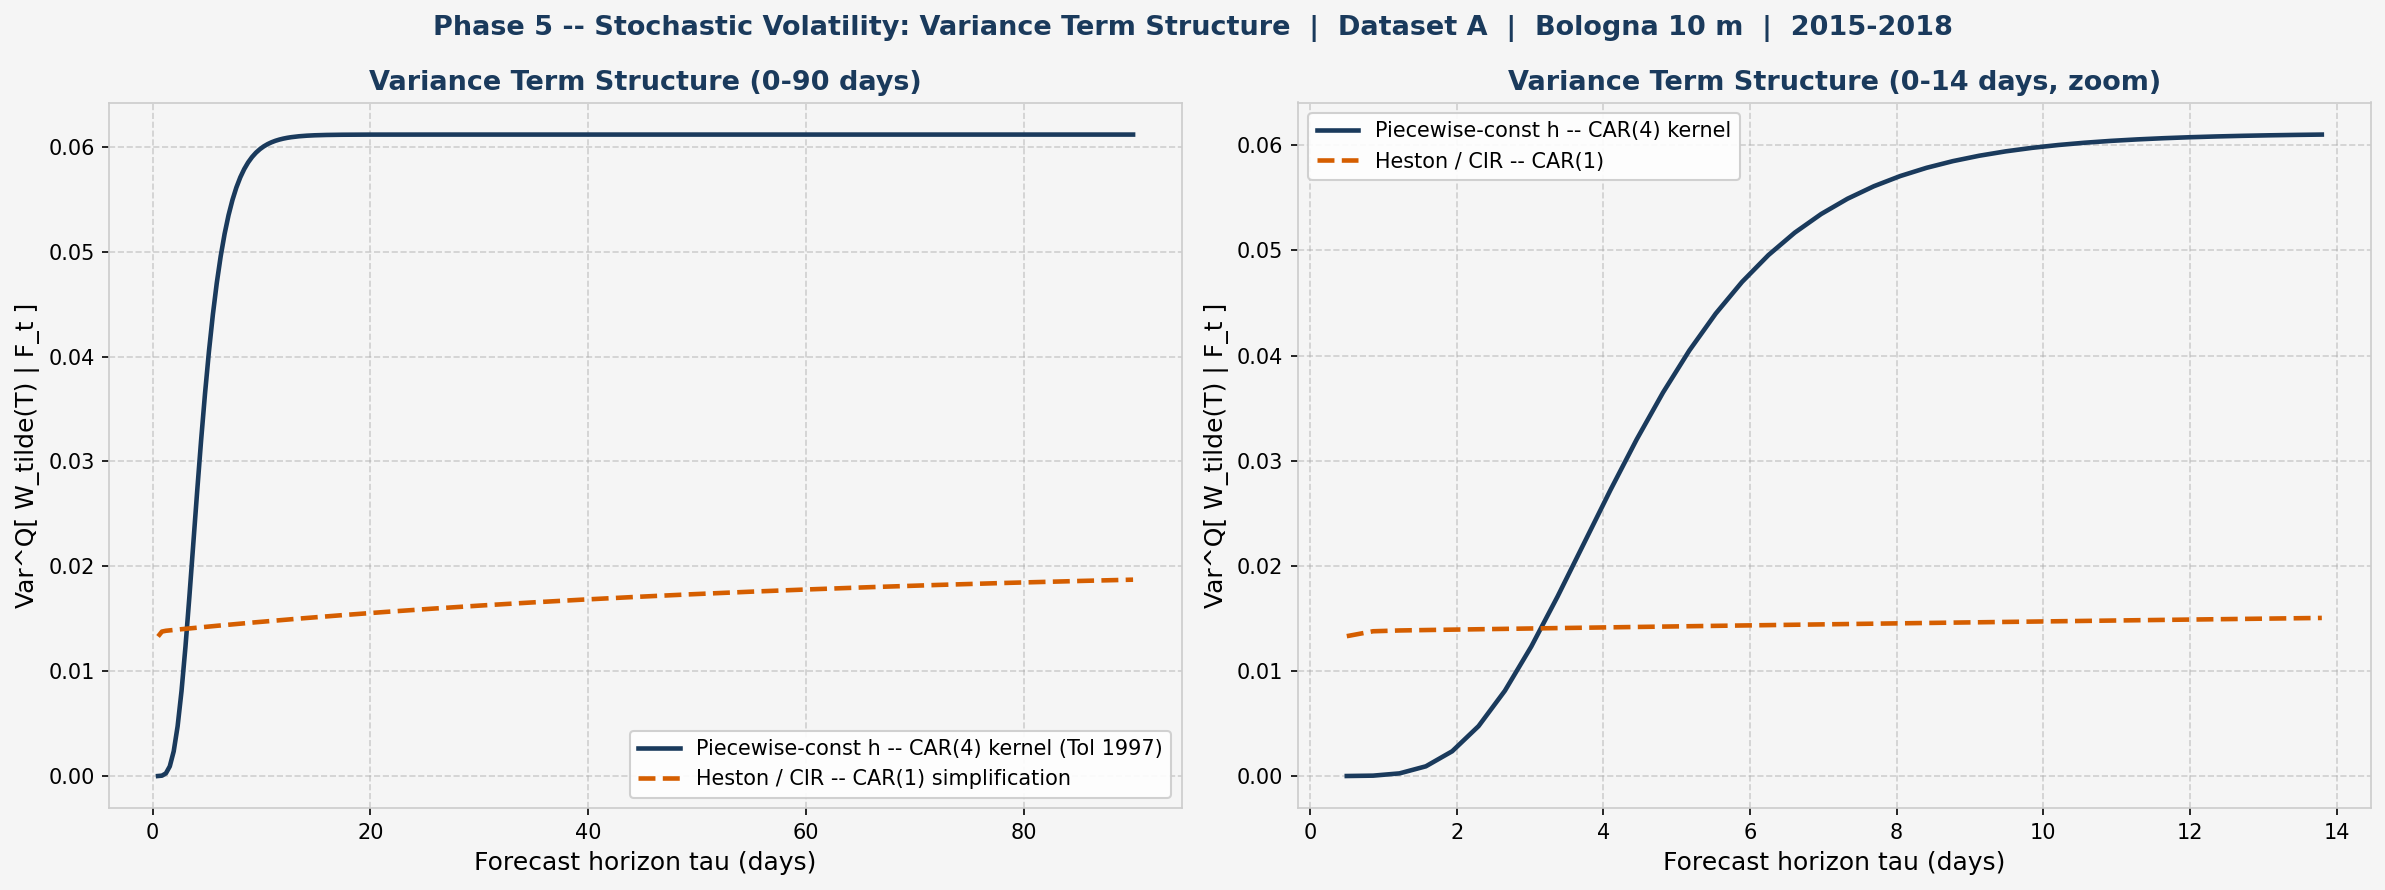
\includegraphics[width=\textwidth]{figures/phase5_A_sv_termstructure.png}
\caption{Dataset A}
\end{subfigure}
\hfill
\begin{subfigure}{0.48\textwidth}
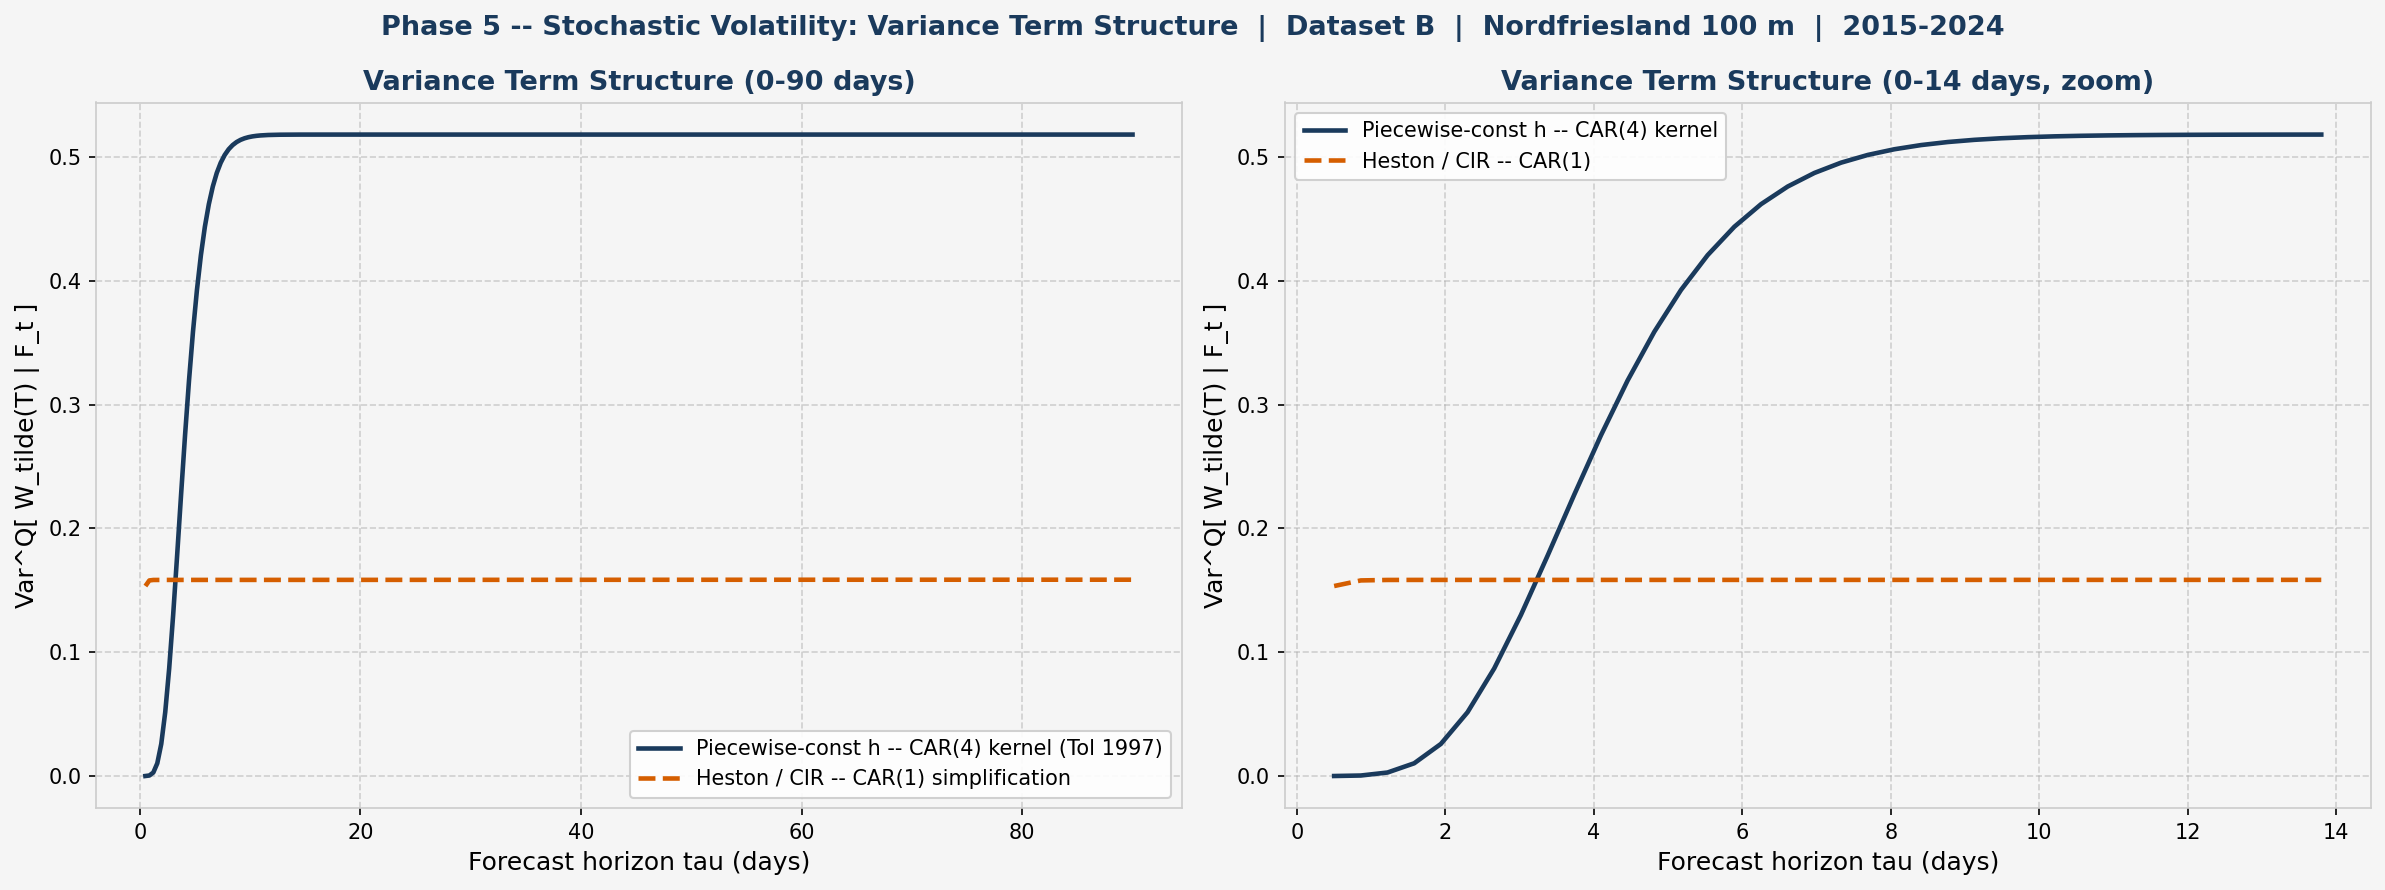
\includegraphics[width=\textwidth]{figures/phase5_B_sv_termstructure.png}
\caption{Dataset B}
\end{subfigure}
\caption{Variance term structure, both datasets: the piecewise-constant-$h$ CAR(4) approximation, following the convention of \citet{Tol1997}, against the simplified Heston/CIR CAR(1) term structure of Section~\ref{sec:phase5-termstructure}. Each panel contains two plots, side by side. \textbf{Left:} the full term structure over a 0--90-day horizon, showing the two approximations converging at long horizons. \textbf{Right:} a zoomed view over 0--14 days, isolating the short-horizon divergence driven by the CAR(4) kernel's $g(0) = 0$ property.}
\label{fig:phase5-termstructure}
\end{figure}

\subsection{Why Maximum-Likelihood Estimation Is Deferred}
\label{sec:phase5-mle}

The CIR parameters $(\kappa_V, \bar v, \xi, \rho)$ above are moment-matching proxies from the GARCH fit, not maximum-likelihood estimates of the continuous-time system itself, and this thesis does not attempt that estimation at daily frequency. The reason is an identification problem inherent to slow-mean-reverting variance processes sampled coarsely relative to their own half-life. With $\kappa_V \approx 0.018$ in both datasets, the implied mean-reversion half-life is on the order of 40 days, so that a daily observation interval provides roughly 40--60 observations per e-folding time; separating the mean-reversion speed $\kappa_V$ from the diffusion coefficient $\xi$ requires enough independent decay cycles to distinguish "reverts slowly with small shocks" from "reverts moderately with occasional large shocks," and at daily frequency the two are close to observationally equivalent. Dataset A compounds this with its short four-year window (1,462 daily observations, of which only a few dozen independent decay cycles are available) and its 10~m measurement height, which would require a further profile correction before any estimated variance dynamics could be applied to hub-height pricing instruments. The designated upgrade path for both datasets is hourly ECMWF ERA5 reanalysis data at the same locations, which would increase the observation count by roughly two orders of magnitude and make the $\xi/\kappa_V$ ratio separately identifiable. Specifically, hourly sampling resolves intraday volatility clustering and the pronounced diurnal cycles of boundary-layer wind speed, high-frequency dynamics that daily aggregation inherently smooths over. Capturing these intraday mechanics is what would allow the diffusion coefficient $\xi$ to be estimated independently of the multi-week synoptic mean-reversion $\kappa_V$, resolving the observational equivalence described above. This is left to future work; for the daily-frequency scope of this thesis, the GARCH-derived proxies under the $\theta=0$, piecewise-constant-$h$ approximation are the operative tool, and are what Chapter~3 uses throughout.

\newpage
\begin{thebibliography}{99}

\bibitem[Alexandridis and Zapranis(2013)]{AlexandridisZapranis2013}
Alexandridis, A., \& Zapranis, A. (2013).
Wind derivatives: modeling and pricing.
\textit{Computational Economics}, 41(3), 299--326.

\bibitem[Barndorff-Nielsen and Shephard(2001)]{BarndorffNielsenShephard2001}
Barndorff-Nielsen, O. E., \& Shephard, N. (2001).
Non-Gaussian Ornstein--Uhlenbeck-based models and some of their uses in financial economics.
\textit{Journal of the Royal Statistical Society: Series B}, 63(2), 167--241.

\bibitem[Benth and \v{S}alty\.{t}\.{e} Benth(2009)]{BenthSaltyteBenth2009}
Benth, F. E., \& \v{S}alty\.{t}\.{e} Benth, J. (2009).
Dynamic pricing of wind futures.
\textit{Energy Economics}, 31(1), 16--24.

\bibitem[Bollerslev(1986)]{Bollerslev1986}
Bollerslev, T. (1986).
Generalized autoregressive conditional heteroskedasticity.
\textit{Journal of Econometrics}, 31(3), 307--327.

\bibitem[Brockwell and Marquardt(2005)]{BrockwellMarquardt2005}
Brockwell, P. J., \& Marquardt, T. (2005).
L\'evy-driven and fractionally integrated ARMA processes with continuous time parameter.
\textit{Statistica Sinica}, 15(2), 477--494.

\bibitem[Diebold and Mariano(1995)]{DieboldMariano1995}
Diebold, F. X., \& Mariano, R. S. (1995).
Comparing predictive accuracy.
\textit{Journal of Business \& Economic Statistics}, 13(3), 253--263.

\bibitem[Engle(1982)]{Engle1982}
Engle, R. F. (1982).
Autoregressive conditional heteroscedasticity with estimates of the variance of United Kingdom inflation.
\textit{Econometrica}, 50(4), 987--1007.

\bibitem[Garcia et al.(1998)Garcia, Torres, Prieto, and de Francisco]{Garcia1998}
Garcia, A., Torres, J. L., Prieto, E., \& de Francisco, A. (1998).
Fitting wind speed distributions: a case study.
\textit{Solar Energy}, 62(2), 139--144.

\bibitem[Haslett and Raftery(1989)]{HaslettRaftery1989}
Haslett, J., \& Raftery, A. E. (1989).
Space-time modelling with long-memory dependence: assessing Ireland's wind power resource.
\textit{Journal of the Royal Statistical Society: Series C (Applied Statistics)}, 38(1), 1--50.

\bibitem[Heston(1993)]{Heston1993}
Heston, S. L. (1993).
A closed-form solution for options with stochastic volatility with applications to bond and currency options.
\textit{Review of Financial Studies}, 6(2), 327--343.

\bibitem[Kavasseri and Seetharaman(2009)]{KavasseriSeetharaman2009}
Kavasseri, R. G., \& Seetharaman, K. (2009).
Day-ahead wind speed forecasting using f-ARIMA models.
\textit{Renewable Energy}, 34(5), 1388--1393.

\bibitem[Schwartz(1997)]{Schwartz1997}
Schwartz, E. S. (1997).
The stochastic behavior of commodity prices: implications for valuation and hedging.
\textit{Journal of Finance}, 52(3), 923--973.

\bibitem[Tol(1997)]{Tol1997}
Tol, R. S. J. (1997).
Autoregressive conditional heteroscedasticity in daily wind speed measurements.
\textit{Theoretical and Applied Climatology}, 56(1--2), 113--122.

\bibitem[Tuller and Brett(1984)]{TullerBrett1984}
Tuller, S. E., \& Brett, A. C. (1984).
The characteristics of wind velocity that favor the Weibull distribution in wind speed analysis.
\textit{Journal of Climate and Applied Meteorology}, 23(1), 124--134.

\end{thebibliography}

\end{document}
